\documentclass[10pt,twocolumn]{article}
\usepackage[margin=0.75in,columnsep=0.28in]{geometry}
\usepackage[T1]{fontenc}
\usepackage{times}
\usepackage{microtype}
\usepackage{amsmath,amssymb}
\usepackage{booktabs}
\usepackage{array}
\usepackage{tikz}
\usetikzlibrary{calc,arrows.meta,positioning}
\usepackage{graphicx}
\usepackage{balance}
\usepackage[breaklinks,hidelinks]{hyperref}
\usepackage{url}

\newtheorem{definition}{Definition}
\newtheorem{proposition}{Proposition}
\newtheorem{condition}{Condition}

\newcommand{\Com}{\mathrm{Com}}
\newcommand{\Rd}{\mathrm{Rd}}
\newcommand{\Sem}{\mathrm{Sem}}
\newcommand{\RQ}[1]{\textbf{RQ#1}}

\setlength{\parindent}{1em}
\raggedbottom

\title{\bf Specification-Driven Software Reconstruction:\\
From Independent Reproduction to Behavioral Discovery}

\author{Rafael Zamora-Resendiz\\
\small Lawrence Berkeley National Laboratory\\
\small \texttt{rzamoraresendiz@lbl.gov}}

\date{Preprint --- October 2026}

\begin{document}
\maketitle

\begin{abstract}
\noindent
Generating a plausible implementation of a software component has become
inexpensive, while establishing what that component is \emph{required} to
do has not. Conventional reproducibility addresses a different question:
given fixed sources, it recovers a fixed artifact. It therefore offers no
account of software whose source is itself generated, and no way to decide
whether a regenerated implementation is the same software as the one it
replaces.

We investigate whether the behavioral requirements of a system are
sufficient to permit independent reconstruction of its implementation. We
introduce a three-machine protocol that separates original production
(M1), byte-preserving transfer (M2), and independent reconstruction from
disclosed requirements alone (M3), together with a content-addressed
identity computed over acceptance requirements while excluding generated
implementation bytes. Repeated reconstruction then becomes an instrument:
implementations admitted by the same requirements are sampled, probed
differentially and against downstream consumers, and the resulting
failures are converted into stronger requirements under explicit human
authorization.

We report results from a system that reconstructs itself and from an
external target. Three reconstructions of a 21-component self-hosting
system qualified at one frozen identity across two producer families,
including one whose kernel operations were executed entirely by a prior
reconstruction; measured cross-family text similarity is 0.123. Six
independent reconstructions of a configuration parser all satisfied its
tests and all broke its consumer identically. On \texttt{jq}, a
conforming reconstruction proved to be a lookup table, and runtime-generated
behavioral laws subsequently closed 15 of 53 consistently divergent probes
against one reopened. Preregistered predictions that failed are reported
as such. One leg of the protocol is itself unmet: no result has been
reproduced by an operator outside the authors' environment, so the
self-hosting evidence demonstrates the protocol's components rather than
a completed instance of it.
\end{abstract}

\section{Introduction}
\label{sec:intro}

Reproducing a computational artifact and reconstructing a software system
are different problems. The first asks whether a byte sequence can be
recovered: given the same sources, toolchain and environment, does the
build produce the same output? Substantial infrastructure now answers
that question well~\cite{lamb2022,dolstra2004,courtes2013}. The second
asks whether the \emph{requirements} that a system satisfies are
sufficient for someone else to build a system that satisfies them too.
That question has received far less attention, because until recently
producing a second independent implementation of anything was expensive
enough that the question was academic.

It is no longer expensive. Large language models now produce syntactically
valid, test-passing implementations of components at a cost low enough to
repeat the exercise many times~\cite{chen2021,austin2021,jimenez2024}.
This changes what can be measured. If an implementation can be regenerated
on demand, then the implementation is no longer the scarce object; the
statement of what it must do is. And if generated implementations are
going to be relied upon, some means is needed of saying what they were
required to do, in a form that can be checked again later, by someone
else, on another machine.

Three observations motivate the work.

\emph{First, source code encodes decisions that its documentation and
tests do not express.} This is an old observation about design
intent~\cite{parnas1986} and about recovering design from artifacts
that no longer explain themselves~\cite{chikofsky1990}. An implementation
resolves questions that nobody wrote down: what happens on a duplicate
key, whether a numeric-looking value is coerced, which inputs are errors.
These resolutions become load-bearing for consumers whether or not they
were ever specified.

\emph{Second, independent implementations can satisfy the same tests and
still disagree on consequential behavior.} The classical diversity
literature established that independently developed programs fail in
correlated ways~\cite{knight1986,eckhardt1985,littlewood1989}. We observe
a sharper version: implementations generated from the same test suite can
agree with each other, pass every test, and be jointly wrong about what a
downstream consumer needs. Agreement among independent implementations is
not evidence of correctness, and in our experiments it was actively
misleading.

\emph{Third, repeated independent reconstruction is now a feasible
experimental procedure.} A specification can be frozen, handed to
several producers that do not see the original implementation, and the
resulting implementations compared against one another, against held-out
observations, and against real consumers. Where they diverge
consequentially, the specification was silent. This turns
underspecification from something discovered by accident in production
into something that can be sampled deliberately in a laboratory.

The research question follows:

\begin{quote}
\emph{Can independent reconstruction serve as an experimental instrument
for measuring and reducing behavioral underspecification?}
\end{quote}

Our approach has two parts. The first is a protocol, the Three-Machine
Test (\S\ref{sec:tmt}), which separates the claim that an artifact
transfers intact from the claim that its requirements suffice to obtain
it. The
second is a loop (\S\ref{sec:discovery}) that uses repeated
reconstruction, differential probing and consumer testing to produce
failure witnesses, and converts witnesses into additional acceptance
requirements under explicit human authorization. Both are implemented in
an open system, \emph{reticuli}~\cite{reticuli}, which serves here as the
experimental platform rather than as the contribution.

\paragraph{Contributions.}
(i) A three-machine protocol that distinguishes artifact verification
from implementation reconstruction, with a three-valued verdict in which
unmeasured conditions can never accept (\S\ref{sec:tmt}). We propose the
protocol and report laboratory evidence for its components; its transfer
leg has not been completed by an independent operator, and by the
protocol's own rule that leaves our self-hosting verdict
\textsf{incomplete} rather than \textsf{accept}.
(ii) An implementation-independent, content-addressed identity defined
over executable acceptance requirements and excluding generated
implementation bytes, with the two conditions its committed byte set must
satisfy (\S\ref{sec:identity}).
(iii) A method for experimentally locating underspecification through
repeated reconstruction, differential probing and consumer substitution
(\S\ref{sec:discovery}).
(iv) Evidence from recursive self-reconstruction and from an external
target that witnessed failures can be converted into stronger acceptance
requirements, with measured effects where they exist and negative results
where they do not (\S\ref{sec:results}).
(v) A framework for studying the cost and reliability of this process,
with the economic questions stated as hypotheses requiring measurement
rather than as findings (\S\ref{sec:discussion}).

We state the support for each claim explicitly. A passing test suite
establishes conformance to that suite. It does not establish semantic
completeness, correctness, or that a producer worked without prior
exposure to the target. Every self-hosting result reported here was
obtained on hardware the authors control, and we mark it accordingly.

\section{Background and Related Work}
\label{sec:related}

\subsection{Reproducible computation and content addressing}

Reproducible builds aim to make the mapping from sources to binaries
deterministic, so that an independent rebuild yields bit-identical
output~\cite{lamb2022}. Functional package managers realize this by
making build inputs explicit and addressing the result by a hash over
them~\cite{dolstra2004,courtes2013}. Bootstrappable builds reduce the
trusted binary seed required to begin~\cite{bootstrappable}. Content
addressing itself, naming data by a hash over its bytes, is
standard~\cite{merkle1987,benet2014}.

All of this fixes the implementation and varies nothing. The guarantee
sought is \emph{identity of artifacts}. Our setting inverts the
quantifiers: the requirements are fixed and the implementation is
permitted, indeed expected, to vary. A reproducible build needs no notion
of which alternative artifacts would have been acceptable, because
exactly one is. Once many artifacts are acceptable, naming requires
deciding which bytes may influence the name, which is the subject of
\S\ref{sec:identity}.

Thompson's argument that a tool's capacity to reproduce itself says
nothing about its trustworthiness~\cite{thompson1984} remains the
relevant caution for any self-hosting result, and diverse
double-compiling~\cite{wheeler2009} is the closest prior method for
attacking it. Our question is adjacent but distinct: not whether an
executable corresponds to its source, but whether fresh source can be
obtained from committed requirements and then perform the work of the
tool that stated them. We eliminate neither the trusted runtime nor the
producer.

\subsection{Specifications and program synthesis}

Executable specifications and contracts have a long
history~\cite{meyer1992,jackson2002}. Inductive program synthesis
constructs programs from examples~\cite{gulwani2011}, and
counterexample-guided inductive synthesis (CEGIS) alternates between
candidate construction and counterexample
generation~\cite{solarlezama2006,alur2013}; counterexample-guided
abstraction refinement (CEGAR) applies the same shape to model
checking~\cite{clarke2000}. Verified compilation relates an
implementation to a formal semantics with machine-checked
proof~\cite{leroy2006,kumar2014}, and regression verification establishes
equivalence between program versions~\cite{godlin2009}.

Our loop is structurally similar to CEGIS and deliberately weaker in what
it concludes. CEGIS refines a candidate against a specification taken as
ground truth. We refine the \emph{specification} against evidence from
candidates, consumers and independent implementations, and the refinement
step is performed by a human who must authorize it. We prove nothing
about semantic equivalence. The output of a successful round is a
specification that excludes a witnessed class of unintended
implementations, not a theorem.

\subsection{Differential, property-based and metamorphic testing}

Differential testing compares implementations of the same interface and
treats disagreement as a bug signal~\cite{mckeeman1998}, with compiler
testing the canonical application~\cite{yang2011}. Property-based
testing~\cite{claessen2000} and metamorphic
testing~\cite{chen1998,segura2016} supply oracles where no reference
output exists, addressing the oracle problem~\cite{barr2015}. Dynamic
invariant inference proposes properties that an existing implementation
appears to maintain~\cite{ernst2007}. Mutation analysis measures the
adequacy of a test suite by its ability to detect seeded
faults~\cite{demillo1978,jia2011}.

We use all of these as components. Two things are different. First, the
implementations being compared are generated rather than independently
developed by separate teams, which makes the comparison cheap and
repeatable but introduces shared priors as a confound (\S\ref{sec:gen}).
Second, the generated-input obligations are placed \emph{inside the
committed identity}, which forces a requirement that is otherwise
optional: the inputs must be drawn from entropy at evaluation time. An
obligation with fixed inputs is a finite test set, and
Proposition~\ref{prop:ext} applies to it.

One difference bounds what a baseline comparison could show, and is
worth stating directly. Differential testing against existing
implementations can find behavioral divergence, and for the divergences
in \S\ref{sec:jq} it plausibly would have. It cannot find that section's
first-generation failure, because that failure is a property of the
\emph{specification} rather than of any existing implementation: the
degenerate member must be constructed before it can be observed, and
constructing it is what generation does. We ran no such comparison and
claim no efficiency advantage; the point is that the two methods have
different reach.

Disagreement locates an investigation target. It does not say which
implementation is right. In our external experiment the reference
implementation was the sole permissive party in one divergence and hung
on another, so "the reference is correct" is not available as a default.

\subsection{Independent implementations and diversity}

N-version programming proposed accepting any of several independently
developed implementations~\cite{avizienis1985}. Knight and Leveson
showed experimentally that independently developed programs fail in
correlated ways~\cite{knight1986}, and the theory of coincident
failures followed~\cite{eckhardt1985,littlewood1989}. The practical
obstacle was always cost.

That obstacle has changed, and the correlated-failure finding has not. It
recurred in our experiments in the strongest available form: six
reconstructions from two unrelated producer families, all conforming, all
breaking a downstream consumer in the same way (\S\ref{sec:substitution}).
Cheap diversity does not purchase independence of judgment.

\subsection{Generative software engineering}
\label{sec:gen}

Benchmarks for code generation measure functional correctness against
test suites~\cite{chen2021,austin2021,hendrycks2021}. Their adequacy has
itself been questioned: strengthening the tests of an existing benchmark
substantially lowers measured pass rates, indicating that the original
suites admitted implementations that were not
correct~\cite{liu2023}. Agentic settings extend this to repository-scale
tasks~\cite{jimenez2024}. Security evaluations of generated code report
systematic defect classes~\cite{pearce2022}. Memorization of training
data is measurable and scales with model
capacity~\cite{carlini2023}, and benchmark contamination is a recognized
threat to evaluation validity~\cite{sainz2023}.

Both the opportunity and the risk in our method come from this
literature. The opportunity is that independent reconstruction is now
affordable enough to run as an experiment. The risk is twofold:
a producer may reproduce a target it has memorized rather than derive it
from the requirements, and two producers may share a prior and thus fail
to be independent in the sense the method needs. We address the first by
withholding the implementation and measuring artifact diversity, and the
second by using two unrelated producer families and reporting
cross-family results separately. Neither measure is conclusive, and
\S\ref{sec:threats} states what remains open.

\subsection{What this work adds}

Relative to reproducible builds: a notion of software identity that
survives reimplementation, with the conditions under which it is sound.
Relative to synthesis: a procedure that treats the specification, not the
candidate, as the object under repair, with human authorization as a
required step. Relative to differential and metamorphic testing: the
placement of generated-input obligations inside a committed identity,
and the use of reconstruction samples rather than existing
implementations as the source of disagreement. Relative to N-version
programming: a demonstration that the correlated-failure problem persists
when versions are generated, and an instrument that detects it through
consumers rather than through mutual comparison. Relative to
code-generation evaluation: a method whose unit of measurement is the
adequacy of the specification rather than the pass rate of a model.

\section{The Three-Machine Test}
\label{sec:tmt}

\begin{figure*}[t]
\centering
% Figure 1 --- The Three-Machine Test.
% Editable TikZ source, sized for a two-column figure* (usable ~17.5cm).
% Layout note: M2 and M3 sit side by side so both carry the same
% symmetric, orthogonal path into the verdict band. Every connector is
% horizontal or vertical. What is withheld from M3 is labelled on its
% own branch rather than drawn as a dangling stub.
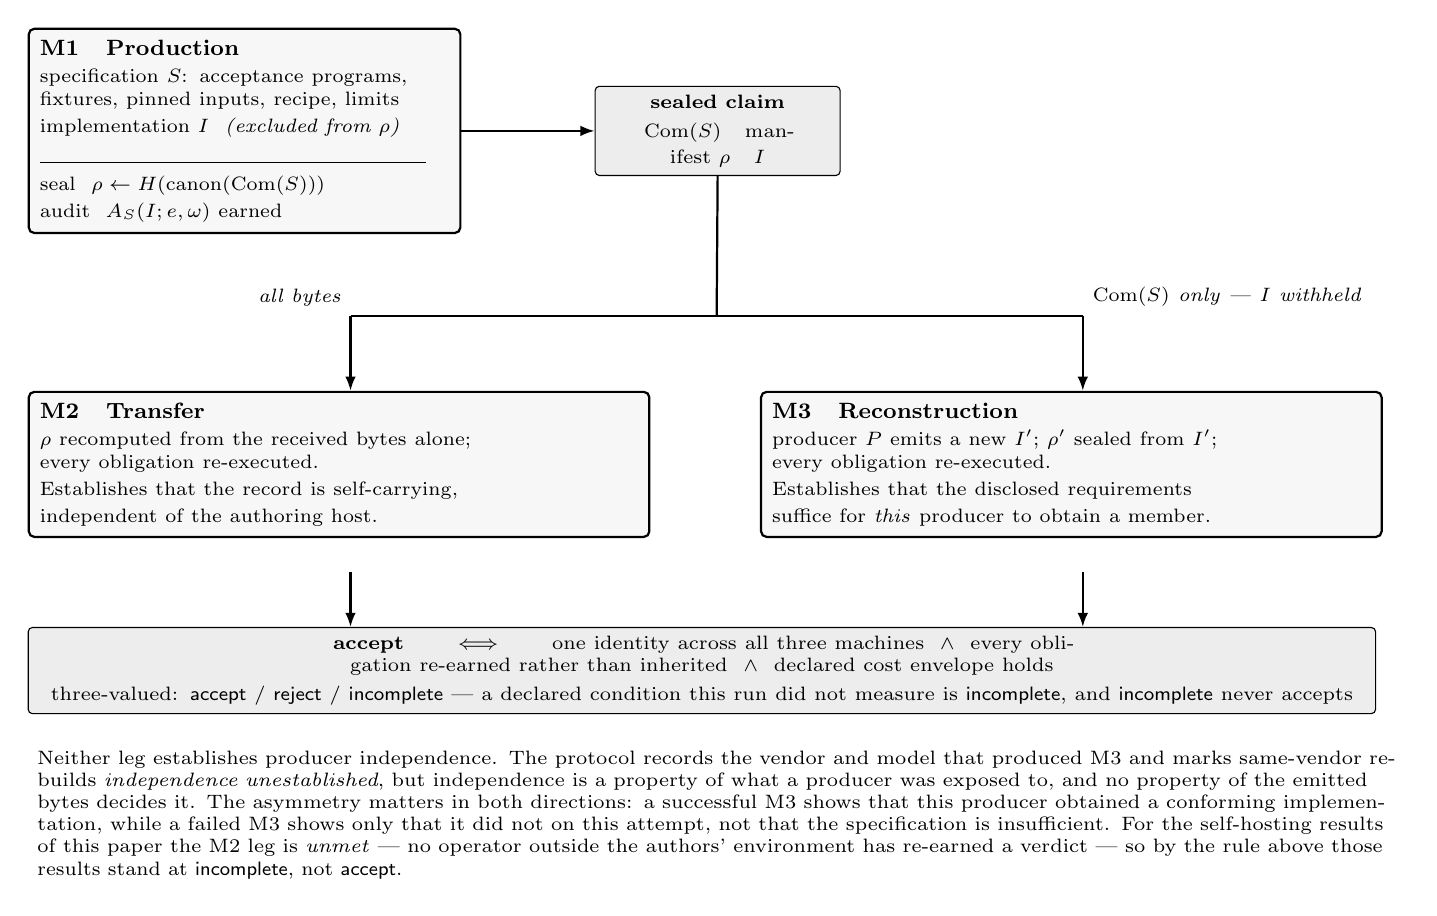
\begin{tikzpicture}[
  font=\footnotesize,
  x=1cm, y=1cm,
  mach/.style={draw, thick, rounded corners=2pt, align=left,
               inner sep=4pt, fill=black!3},
  pass/.style={draw, rounded corners=1.5pt, align=center,
               inner sep=3pt, fill=black!7},
  flow/.style={-{Latex[length=1.8mm]}, thick},
  bus/.style={thick},
  tag/.style={font=\scriptsize\itshape, inner sep=2pt},
  ev/.style={font=\scriptsize, align=left},
]

% ---------------------------------------------------------------- M1
\node[mach, text width=5.2cm, anchor=west] (m1) at (0,0) {%
  \textbf{M1\quad Production}\\[2pt]
  \scriptsize
  specification $S$: acceptance programs,\\
  fixtures, pinned inputs, recipe, limits\\[2pt]
  implementation $I$ \ \emph{(excluded from $\rho$)}\\[3pt]
  \rule{4.9cm}{0.3pt}\\[2pt]
  seal \ $\rho \leftarrow H(\operatorname{canon}(\Com(S)))$\\
  audit \ $A_S(I;e,\omega)$ earned};

% ------------------------------------------------- transmitted object
\node[pass, text width=2.9cm, anchor=west] (claim) at (7.2,0) {%
  \scriptsize\textbf{sealed claim}\\[1pt]
  $\Com(S)$ \ \ manifest $\rho$ \ \ $I$};

\draw[flow] (m1.east) -- (claim.west);

% ----------------------------------------------- the fan-out, as a bus
\draw[bus] (claim.south) -- (8.75,-2.35);
\draw[bus] (4.10,-2.35) -- (13.40,-2.35);
\draw[flow] (4.10,-2.35) -- (4.10,-3.30);
\draw[flow] (13.40,-2.35) -- (13.40,-3.30);

\node[tag, anchor=south east] at (4.05,-2.30) {all bytes};
\node[tag, anchor=south west] at (13.45,-2.30)
  {$\Com(S)$ only --- $I$ withheld};

% ------------------------------------------------------------ M2 / M3
\node[mach, text width=7.6cm, anchor=north west] (m2) at (0.0,-3.30) {%
  \textbf{M2\quad Transfer}\\[2pt]
  \scriptsize
  $\rho$ recomputed from the received bytes alone;\\
  every obligation re-executed.\\[2pt]
  Establishes that the record is self-carrying,\\
  independent of the authoring host.};

\node[mach, text width=7.6cm, anchor=north west] (m3) at (9.30,-3.30) {%
  \textbf{M3\quad Reconstruction}\\[2pt]
  \scriptsize
  producer $P$ emits a new $I'$; $\rho'$ sealed from $I'$;\\
  every obligation re-executed.\\[2pt]
  Establishes that the disclosed requirements\\
  suffice for \emph{this} producer to obtain a member.};

% ------------------------------------- symmetric drops into the verdict
\draw[flow] (4.10,-5.60) -- (4.10,-6.30);
\draw[flow] (13.40,-5.60) -- (13.40,-6.30);

\node[pass, text width=16.9cm, anchor=north west] (v) at (0,-6.30) {%
  \scriptsize
  \textbf{accept} $\iff$ one identity across all three machines
  \ $\wedge$ \ every obligation re-earned rather than inherited
  \ $\wedge$ \ declared cost envelope holds\\[1pt]
  three-valued: \textsf{accept} / \textsf{reject} /
  \textsf{incomplete} --- a declared condition this run did not measure
  is \textsf{incomplete}, and \textsf{incomplete} never accepts};

% ------------------------------------------------------------- caveat
\node[ev, anchor=north west, text width=17.3cm] at (0,-7.75) {%
  Neither leg establishes producer independence. The protocol records
  the vendor and model that produced M3 and marks same-vendor rebuilds
  \emph{independence unestablished}, but independence is a property of
  what a producer was exposed to, and no property of the emitted bytes
  decides it. The asymmetry matters in both directions: a successful M3
  shows that this producer obtained a conforming implementation, while a
  failed M3 shows only that it did not on this attempt, not that the
  specification is insufficient. For the self-hosting results of this
  paper the M2 leg is \emph{unmet} --- no operator outside the authors'
  environment has re-earned a verdict --- so by the rule above those
  results stand at \textsf{incomplete}, not \textsf{accept}.};

\end{tikzpicture}

\caption{The Three-Machine Test. M2 and M3 answer different questions.
M2 receives every byte and establishes that identity and verdicts survive
transport. M3 receives the committed requirements only and establishes
that they determine a conforming implementation. The protocol records
information relevant to producer independence but cannot establish it
from program bytes.}
\label{fig:tmt}
\end{figure*}

A \emph{claim} is a specification together with its sealed evidence: the
executable acceptance obligations, the inputs they are pinned to, the
recipe describing which outputs are generated and how, reproducibility
metadata, and the generated implementation artifacts themselves. The
protocol evaluates a claim on three machines.

\paragraph{M1 --- production.} The original environment. An
implementation is produced, the acceptance obligations are executed
against it, and the claim is sealed: its identity is computed and
recorded in a manifest.

\paragraph{M2 --- transfer.} A byte-preserving copy of the claim is
exported, imported into a different environment, and checked there. The
identity is recomputed from the received bytes alone and compared with
the manifest, and the acceptance obligations are re-executed.

\paragraph{M3 --- independent reconstruction.} A workspace is
materialized containing the committed material only: obligations,
fixtures, pinned inputs and recipe. The original implementation is not
present. A producer generates a new implementation, which is then sealed
and judged.

The distinction between M2 and M3 is the point of the protocol. M2 tests
whether a record is self-carrying: whether the evidence travels without
the authoring host. This is the property reproducible-build infrastructure
is designed to provide, and a failure of M2 is a defect in packaging or
in the identity computation. M3 tests whether the disclosed requirements
are sufficient for the tested producer to obtain a conforming
implementation.

The two directions are not symmetric, and we state the asymmetry because
our results depend on it. A successful M3 establishes that \emph{this}
producer obtained an implementation satisfying the obligations as
evaluated. A failed M3 establishes only that this producer did not, on
this attempt, within the resources allowed; a complete specification can
still defeat a producer that lacks the capability, context or attempts
to satisfy it. Diagnosis requires reading the failure. Where we treat a
failure as evidence about the specification, as in
\S\ref{sec:substitution} and \S\ref{sec:jq}, it is because the failing
behavior was traced to a requirement the specification did not state,
not because a reconstruction failed.

\subsection{The verdict}

A crosscheck accepts when one identity holds across all three machines,
every obligation is re-earned rather than inherited from a record, and
the declared cost envelope holds. The cost comparison uses the strongest
unit both M1 and M3 recorded, in the order
$\mathtt{usd} > \mathtt{tokens} > \mathtt{calls} > \mathtt{seconds}$;
the default tolerance on the M3-to-M1 ratio is $2.0$, and a claim or a
verifier may set any value in $[1.5, 4.0)$. Where a claim declares a
mutation floor, M3 must re-earn that too, with deterministic mutants
drawn from the identity and a required kill rate.

The monetary unit needs a caveat that our own runs make concrete, and it
is worth separating two mechanisms that are easily conflated. The cost
\emph{band} compares two ledgers and so may descend the ladder to any
unit both machines recorded. The declared \emph{envelope} compares a
measurement against a ceiling the claim states in one particular unit,
where descending the ladder would be wrong: a ceiling in dollars is not
a statement about tokens, and substituting one for the other would
manufacture a comparison the claim never declared.

Both producer families here ran on flat-rate subscriptions, which do not
expose a marginal monetary figure. The protocol's rule is that an absent
measurement means unmeasured and that unmeasured is never written as
zero, so a reader can always distinguish \emph{free} from
\emph{unknown}. Our producer adapters follow it: they record tokens and
elapsed time, omit \texttt{usd} entirely, and note the un-metered
source. No run in the artifact records a monetary figure of any value.
The declared \$40 ceiling therefore compares against an absent
measurement, yields \textsf{incomplete} by the three-valued rule below,
and never accepted (\S\ref{app:measurements}). The condition is reported
as unmeasured because it \emph{is} unmeasured, not because we chose to
present it that way.

The verdict is three-valued: \textsf{accept}, \textsf{reject},
\textsf{incomplete}. A hard condition must hold to accept and rejects on
failure. A hard condition that the claim declared but that this run did
not measure is neither satisfied nor violated, and the verdict is
\textsf{incomplete}. Incomplete never accepts. The rule exists because
the common failure of verification tooling is to treat an unmeasured
condition as a satisfied one, and the distinction between \emph{missing
evidence} and \emph{rejection} is exactly what a reader of a verdict
needs.

\subsection{What the protocol does not establish}

The protocol records which vendor and model produced M3 and marks
same-vendor rebuilds as \emph{independence unestablished}. It does not
and cannot establish producer independence. Independence is a property of
what a producer was exposed to, and no property of the emitted bytes
decides it. We therefore treat the blindness of a reconstruction as a
declared protocol with indirect support --- the harness does not route
the original implementation into the workspace, the resulting artifacts
are measurably dissimilar (\S\ref{sec:selfhost}), and two unrelated
producer families are used --- and not as a verified fact. A successful
reconstruction is an observation. It is not a proof that the producer had
no prior exposure to the target.

\section{Implementation-Independent Identity}
\label{sec:identity}

\subsection{Construction}

Let a specification $S$ be a finite map from paths to byte strings, each
path carrying a declared role. Let an implementation $P$ be the material
a producer supplies. An acceptance procedure evaluates an implementation
under a declared execution environment $e$ and, where obligations draw
generated inputs, a seed $\omega$:
\begin{equation}
A_S(P;e,\omega) \in \{0,1\}.
\label{eq:accept}
\end{equation}

The seed is not a formality. Section~\ref{sec:discovery} requires it to
be drawn fresh at each evaluation, so acceptance is a property of a
\emph{run}, not of an implementation alone. Two notions must therefore
be separated. The verdict of a particular audit is
$A_S(P;e,\omega)$. The set of implementations a specification admits
\emph{without qualification} is

\begin{equation}
\mathcal{I}(S) \;=\; \{\,P \;\mid\; A_S(P;e,\omega) = 1
  \ \text{for all } \omega\,\},
\label{eq:admitted}
\end{equation}

which is not observable: no finite number of audits establishes
membership. What an audit establishes is one draw. We therefore write

\begin{equation}
\widehat{\mathcal{I}}(S) \;=\; \{\,P \;\mid\; A_S(P;e,\omega) = 1
  \ \text{for every } \omega \text{ evaluated}\,\}
\label{eq:observed}
\end{equation}

for the \emph{observed} admitted set, and use it for every experimental
result in this paper. Every implementation we report as admitted belongs
to $\widehat{\mathcal{I}}$, and $\widehat{\mathcal{I}}(S) \supseteq
\mathcal{I}(S)$, so observed admission is the weaker statement. The
useful quantity for an unevaluated future audit is a pass
\emph{probability} rather than a guarantee, and we make no claim about
it, having run too few draws per implementation to estimate one.

The identity is a hash over a declared subset of the specification's
bytes,

\begin{equation}
\rho(S) \;=\; H\!\left(\operatorname{canon}\big(\{(p, H(S[p])) : p \in \Pi(S)\}\big)\right),
\label{eq:root}
\end{equation}

where $\Pi(S)$ is the \emph{committed path set} and $\operatorname{canon}$
a canonical encoding. We write $\Com(S)$ for the committed content.
Generated implementation bytes are excluded from $\Pi(S)$ by
construction: in our implementation the identity computation skips every
path whose declared class is \emph{generated}. That exclusion is the
mechanism by which $\rho$ names $\mathcal{I}(S)$ rather than any member
of it.

\subsection{Two conditions on the committed set}

Choosing $\Pi(S)$ is the whole difficulty, and it is constrained from
two sides. Define the \emph{read set} $\Rd(A,S)$ as the set of
specification paths whose contents can change the outcome of $A_S$ on
some implementation, and $\Sem(S)$ as the paths carrying semantic
content, as opposed to presentation.

\begin{condition}[Determination]
\label{cond:det}
For all $S_1, S_2$, all $P$, and every $e$ and $\omega$:
$\rho(S_1) = \rho(S_2) \Rightarrow
A_{S_1}(P;e,\omega) = A_{S_2}(P;e,\omega)$.
\end{condition}

Determination holds if and only if $\Rd(A,S) \subseteq \Pi(S)$ for every
$S$, under three assumptions we state because they are load-bearing:
that $A_S$ is deterministic given its declared execution environment and
seed, that the environment is fixed across the comparison, and that $H$
is collision-resistant, so that equal identities imply equal committed
content. The necessity direction is immediate: if some path outside $\Pi$ can
influence an outcome, then two specifications differing only there share
an identity and disagree on a verdict.

This failed in our system in an instructive form. Producer guidance ---
prose attached to a generated output, addressed to whoever writes it ---
had been removed from the committed set for reasons given below. The
judging workspace, however, was still materialized from the \emph{raw}
specification, guidance included. An acceptance program that read its own
guidance could therefore accept differently under one identity. Our
documentation asserted this was impossible; a reproduction showed that as
implemented it was not.

\begin{condition}[Admissibility]
\label{cond:adm}
If $S_1$ and $S_2$ differ only on paths outside $\Pi(S)$, then
$\rho(S_1) = \rho(S_2)$.
\end{condition}

This is invariance under excluded material, and it holds by construction
for any $\Pi$. Its content is therefore entirely in the choice of $\Pi$:
the smaller the committed set, the more verdict-irrelevant material the
identity ignores. Determination bounds how small it may be, so the design
goal is
\begin{equation}
\Pi(S) \;=\; \Rd(A,S),
\label{eq:equality}
\end{equation}
committing every acceptance-relevant path and no other.

Two caveats attach to \eqref{eq:equality} as an engineering target.
Computing the exact read set of an arbitrary executable acceptance
program is not tractable in general, and our implementation does not
attempt it: it declares a committed boundary and enforces it by
construction, materializing only committed content into the context in
which obligations execute. The equality is approached by restricting
what the evaluator can reach, not derived by analysis. And the
invariance in Condition~\ref{cond:adm} assumes that editing excluded
material does not itself change which paths are committed, which holds
here because the committed set is declared in material that is itself
committed.

We state the condition this way because the stronger form is
unobtainable, and an earlier version of this paper asserted it. One
might want: if $S_1$ and $S_2$ admit the same implementations, then
$\rho(S_1) = \rho(S_2)$. No choice of $\Pi$ delivers that. Both $\Pi$ and
$\Rd$ are sets of \emph{paths}, while verdict-irrelevant variation also
occurs \emph{within} a path. Adding a comment to a committed acceptance
program changes no verdict and leaves the read set identical, yet changes
the bytes at a committed path and so changes the identity. Delivering
invariance there would require canonicalizing programs up to semantic
equivalence, which is not available in general. We therefore claim path
discipline, not semantic canonicalization.

The residue is not hypothetical, and it has cost us. A comment-only
change to a committed obligation moved an identity, and under the strict
reading of the no-intervening-change condition that invalidated a trial
which had already qualified; it was regrown at the new identity
(\S\ref{sec:selfhost}). That is this limitation in production.

Where the irrelevant structure is \emph{known and finitely describable},
partial canonicalization recovers some of the gap, and both of our
witnesses below are of that kind. They work because they canonicalize a
specific construct in the preimage, not because they decide equivalence.

A violation of the condition does not produce a wrong verdict;
it produces a wrong \emph{name}. An implementation
satisfies every obligation, receives a different identity, and is
rejected as a different thing. We observed this twice. First with prose:
an independently written packager, conforming in every behavioral
respect, phrased generated guidance differently and minted a different
identity for an entire dependency chain. Second with order: once prose
was removed, the residue was sequence. The step list was committed as a
list, and two conforming packagers enumerated the same steps in
different orders --- one lexicographic, one following glob expansion ---
drifting 13 of 20 chain identities. The committed encoding now sorts
steps canonically, making the list a set.

Both witnesses are instances of the same move: material was taken
\emph{out} of $\Pi$, or canonicalized within it, once it was shown to
carry no verdict. Neither widened the committed set.

Three notions must be kept apart here, and conflating them is the error
we made. A path may be \emph{semantically relevant} --- carrying
real information about what is wanted --- without being
\emph{acceptance-relevant}. Producer guidance is exactly such material:
it tells an implementer what is intended and, by design, must never
change a verdict. Writing $G(S)$ for guidance, the design constraint is
$G(S) \subseteq \Sem(S) \setminus \Rd(A,S)$, and \eqref{eq:equality}
then excludes guidance from the identity automatically. An earlier
formulation of ours placed $\Sem(S)$ as an upper bound on $\Pi(S)$ and
described the gap between $\Rd$ and $\Sem$ as designer freedom. That was
wrong: admissibility as stated admits no such gap, because material
that cannot change a verdict must not be committed whether or not it is
meaningful.

The practical consequence survives the correction, and is the reason the
obvious repair to a determination failure is the wrong one. When a byte
must be excluded for admissibility yet the acceptance program can read
it, widening $\Pi$ is unavailable. The only sound repair is to shrink
$\Rd$ --- to make the byte \emph{unreadable} by separating the context
in which an implementation is constructed from the context in which it
is judged. In our system the judging workspace is now materialized from
the committed content itself, so no acceptance program can read what the
identity does not cover.

\subsection{Composition}

Specifications depend on other specifications. Let $C$ declare edges
$(d,o,i)$ meaning that component $d$ supplies output $o$ to $C$'s input
$i$, and let $C$ ship bytes $\beta_C(i)$ at that input. The composed
verdict must be

\begin{equation}
A^{*}(C) \;=\; A_C \;\wedge\!\! \bigwedge_{(d,o,i)}\! A_{D_d}\big(\beta_C(i) \text{ as } o\big).
\label{eq:compose}
\end{equation}

Each component's own acceptance procedure is re-executed on the bytes the
dependent actually ships. A recorded verdict from the component's history
is not evidence about the dependent's bytes, because the component's
identity names a class and the dependent links one member of it.

Equation~\eqref{eq:compose} was violated in three places in our
implementation, each exploitable. A dependency attribution recorded at
seal time and never re-checked allowed a claim to assert an origin its
bytes did not have, and the forged claim passed identity verification,
shallow acceptance, composed acceptance and the dependency view in every
implementation we tested, including the reference one. A signing
ceremony folded every declared component into the signed identity while
re-earning only $A_C$, so a claim whose own composed audit rejects it
could be signed. And the user-facing audit verb resolved to composed
acceptance by behavior alone, with no obligation requiring it, so a
reconstruction was free to wire the verb to the shallow primitive and
pass every test.

The three share a structure. In each case the obligations exercised one
side of a two-sided contract: code edges were re-earned but data edges
were not; the signing ceremony's refusal behavior was tested but its
composed refusal was not; the verb's denial behavior was pinned but its
permission behavior was not. This generalizes into an audit procedure.
To look for omissions in a specification, enumerate the symmetries of its
contracts and check whether both halves are exercised.

\subsection{Test-based and behavioral equivalence}

Equation~\eqref{eq:admitted} defines equivalence relative to an
acceptance procedure, which is weaker than behavioral equivalence and
must not be confused with it. $\mathcal{I}(S)$ can contain mutually
incompatible implementations whenever $A_S$ omits a requirement that
some consumer depends on. Section~\ref{sec:substitution} exhibits exactly
this: six implementations, all in $\widehat{\mathcal{I}}(S)$, none usable
by the consumer. An identity over $S$ therefore names \emph{a declared
experiment}, not a semantic property of programs. Two specifications that
test the same behavior by different means receive different identities;
identity equality asserts the same question, not the same answer.

\subsection{Specification transitions}

Strengthening or otherwise changing the obligations produces a new
identity. Our implementation treats this as a deliberate, recorded,
human-authorized act: the lineage of revisions is retained, each
transition names the failure that motivated it, and no automated step may
perform one. The practical significance for the experiments below is that
adopting a new obligation invalidates prior qualifying results at the old
identity, which is why the counts in \S\ref{sec:selfhost} reset as often
as they do.

\section{Reconstruction as Specification Discovery}
\label{sec:discovery}

\begin{figure}[t]
\centering
% Figure 2 --- The specification refinement loop.
% Editable TikZ source. Sized for a single-column figure (usable width
% ~8.4cm). The feedback edge returns to a NEW specification version; it
% never mutates the frozen one. Authorization is drawn as a distinct,
% human-held step because no automated step may move an identity.
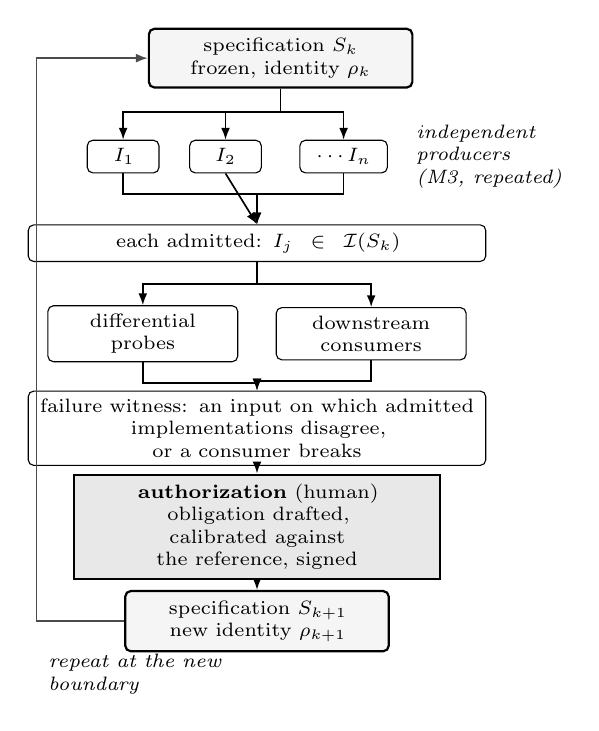
\begin{tikzpicture}[
  font=\scriptsize,
  x=1cm, y=1cm,
  stage/.style={draw, rounded corners=2pt, align=center, inner sep=3pt},
  spec/.style={draw, thick, rounded corners=2pt, align=center,
               inner sep=3.5pt, fill=black!4},
  auth/.style={draw, thick, align=center, inner sep=3.5pt, fill=black!9},
  flow/.style={-{Latex[length=1.5mm]}, semithick},
  back/.style={-{Latex[length=1.5mm]}, semithick, draw=black!70},
  note/.style={font=\scriptsize\itshape, align=left},
]

% -------------------------------------------------- frozen specification
\node[spec, text width=3.1cm] (s) at (0,0)
  {specification $S_k$\\frozen, identity $\rho_k$};

% ---------------------------------------------------- reconstructions
\node[stage, text width=0.7cm] (r1) at (-2.0,-1.25) {$I_1$};
\node[stage, text width=0.7cm] (r2) at (-0.7,-1.25) {$I_2$};
\node[stage, text width=0.9cm] (r3) at ( 0.8,-1.25) {$\cdots I_n$};

\draw[flow] (s.south) -- ++(0,-0.30) -| (r1.north);
\draw[flow] (s.south) -- ++(0,-0.30) -| (r2.north);
\draw[flow] (s.south) -- ++(0,-0.30) -| (r3.north);

\node[note, anchor=west] at (1.6,-1.25) {independent\\producers\\(M3, repeated)};

% ------------------------------------------------------------ admitted
\node[stage, text width=5.6cm] (adm) at (-0.3,-2.35)
  {each admitted: $I_j \in \mathcal{I}(S_k)$};

\draw[flow] (r1.south) |- ++(0,-0.26) -| (adm.north);
\draw[flow] (r2.south) -- (adm.north);
\draw[flow] (r3.south) |- ++(0,-0.26) -| (adm.north);

% -------------------------------------------------------------- probes
\node[stage, text width=2.2cm] (diff) at (-1.75,-3.50)
  {differential\\probes};
\node[stage, text width=2.2cm] (cons) at ( 1.15,-3.50)
  {downstream\\consumers};

\draw[flow] (adm.south) -- ++(0,-0.28) -| (diff.north);
\draw[flow] (adm.south) -- ++(0,-0.28) -| (cons.north);

% ------------------------------------------------------------- witness
\node[stage, text width=5.6cm] (w) at (-0.3,-4.70)
  {failure witness: an input on which admitted\\
   implementations disagree, or a consumer breaks};

\draw[flow] (diff.south) |- ++(0,-0.26) -| (w.north);
\draw[flow] (cons.south) |- ++(0,-0.26) -| (w.north);

% -------------------------------------------------------- authorization
\node[auth, text width=4.4cm] (a) at (-0.3,-5.95)
  {\textbf{authorization} (human)\\
   obligation drafted, calibrated against\\
   the reference, signed};

\draw[flow] (w.south) -- (a.north);

% ---------------------------------------------------- new specification
\node[spec, text width=3.1cm] (s2) at (-0.3,-7.15)
  {specification $S_{k+1}$\\new identity $\rho_{k+1}$};

\draw[flow] (a.south) -- (s2.north);

% the loop edge, returning as a NEW version
\draw[back] (s2.west) -- (-3.1,-7.15) -- (-3.1,0) -- (s.west);
\node[note, anchor=north west, text width=2.5cm] at (-3.05,-7.45)
  {repeat at the new boundary};

\end{tikzpicture}

\caption{The specification refinement loop. Independent reconstructions
sample $\widehat{\mathcal{I}}(S_k)$; differential probes and downstream
consumers
produce failure witnesses; an authorized refinement yields a new
specification version $S_{k+1}$ with a new identity. The frozen
specification is never mutated in place.}
\label{fig:loop}
\end{figure}

Repeated independent reconstruction samples $\widehat{\mathcal{I}}(S)$.
If the
sampled implementations disagree consequentially, or if any of them
breaks a consumer that the original satisfied, then $A_S$ omits a
requirement. The loop in Figure~\ref{fig:loop} makes this a procedure:

\begin{enumerate}\itemsep1pt
\item Freeze a specification and its acceptance boundary.
\item Generate independent candidate implementations (M3, repeated).
\item Confirm that each is admitted by the frozen boundary.
\item Probe the candidates against held-out observations, downstream
      consumers, and generated behavioral probes.
\item Identify consequential divergence or consumer failure, and retain
      the witnessing input.
\item Convert justified witnesses into additional acceptance
      obligations, calibrated against the reference before adoption.
\item Seal the revised specification under a new identity, and repeat.
\end{enumerate}

\subsection{Measured quantities}

The loop defines several measurable quantities: the acceptance rate of
independent reconstructions at a boundary; cross-implementation
disagreement, measured per probe; consumer compatibility, measured as the
fraction of admitted implementations a consumer can use; reconstruction
cost in the units the producer reports; the distribution of failure
classes; and the change in disagreement following a repair. The last of
these is the one most easily measured wrongly, and
\S\ref{sec:jq} reports an instance in which we did so.

\subsection{Two limits of the instrument}

\paragraph{Agreement is not correctness.} Producers may share an
interpretation, in which case the sampled implementations converge on a
reading that is uniformly wrong. This is the correlated-failure
result~\cite{knight1986} reappearing with generated versions, and it
bounds what mutual comparison can find. Only an external
oracle --- a consumer, a reference implementation, a human
judgment --- can detect a shared error. Our strongest instance is in
\S\ref{sec:substitution}.

\paragraph{Finite test sets admit memorization.}

\begin{proposition}[Extensional insufficiency]
\label{prop:ext}
Let $S$ have acceptance obligations consisting of a finite set of
input-output observations $\{(x_j,y_j)\}_{j \le n}$ compared exactly.
Then $\mathcal{I}(S)$ contains an implementation of size $O(n)$ --- the
universal set, since with a fixed finite corpus there is no seed to vary
--- that
stores the observations, answers $y_j$ on $x_j$, and is unconstrained on
every other input.
\end{proposition}

The proposition is trivial as mathematics. It is reported because the
degenerate member is not hypothetical; \S\ref{sec:jq} records a
reconstruction that realized it, documented what it had done, and passed.
The repair is to add obligations whose inputs do not exist when the
implementation is written: computed relations, in which the checker
derives the expected result independently for each generated input;
metamorphic relations between executions, which need no
oracle~\cite{chen1998}; and refusal obligations, in which generated
ill-typed inputs must raise, guarded so that refusing everything cannot
satisfy them.

These do not categorically exclude table-based strategies, and we do not
claim they do. They change the economics. Memorizing the original finite
corpus no longer suffices, because the inputs that decide the verdict do
not exist when the implementation is written; a table would have to
cover the generator's reachable input space, which for the obligations
we use is far larger than the corpus and in the limit unbounded. The
degenerate member is made expensive rather than impossible, and an
implementation that memorized the \emph{generator} would still defeat
them.

Two consequences follow, both learned the hard way. The entropy must be
drawn fresh at each evaluation; a fixed seed converts the obligations
into a larger finite test set, and Proposition~\ref{prop:ext} applies
again. And each obligation must be calibrated against the reference
before it is committed, because an obligation that misstates the
reference's behavior refuses conforming implementations
(\S\ref{sec:jq}).

\section{Experimental Design}
\label{sec:design}

\begin{table*}[t]
\centering\small
\caption{Experimental design. No experiment was run for this manuscript;
all were conducted during the development of the platform, and the
preregistration applies to the \texttt{jq} arm only.}
\label{tab:design}
\begin{tabular}{@{}p{0.155\textwidth}p{0.20\textwidth}p{0.20\textwidth}p{0.37\textwidth}@{}}
\toprule
& target & producers & outcome measure \\
\midrule
\RQ{1} independent reconstruction
  & 21-component self-hosting system
  & codex, claude
  & acceptance at frozen identity; artifact similarity \\[2pt]
\RQ{2} recursive self-hosting
  & the same, generationally
  & codex authored, claude executing
  & identity preserved with kernel acts performed by a reconstruction \\[2pt]
\RQ{3} underspecification
  & configuration parser with a consumer
  & 3 codex models, 3 claude models
  & admitted implementations that break the consumer \\[2pt]
\RQ{4} specification repair
  & self-hosting system; \texttt{jq}
  & both families
  & new failures per generation; paired per-probe divergence \\[2pt]
\RQ{5} generalization
  & \texttt{jq} 1.8.1 (external)
  & codex, claude
  & divergence recall against an independent human-divergence surface \\
\bottomrule
\end{tabular}
\end{table*}

We organize the evidence around five questions (Table~\ref{tab:design}).

\RQ{1} \emph{Independent reconstruction.} Can distinct implementations
satisfy the same sealed specification without reusing the original
implementation?

\RQ{2} \emph{Recursive self-hosting.} Can a reconstructed implementation
perform the verification and reconstruction operations required to
produce subsequent implementations?

\RQ{3} \emph{Underspecification.} Do independent reconstructions and
external consumers expose behavioral obligations missing from the
acceptance criteria?

\RQ{4} \emph{Specification repair.} Can witnessed failures be converted
into requirements that reduce measurable consequential divergence?

\RQ{5} \emph{Generalization.} Does the method reveal useful
underspecification in independently developed external software?

\paragraph{Producers and environments.} Two unrelated producer families
were used throughout: a \emph{codex} family (models recorded as
\texttt{gpt-6-sol}, with \texttt{gpt-6-luna} and \texttt{gpt-6-astra} in
the substitution experiment) and a \emph{claude} family (\texttt{sonnet},
with \texttt{opus} and \texttt{haiku} in the substitution experiment).
Reconstruction ran on a single \texttt{arm64} Darwin host with
CPython 3.14, acceptance obligations executed under a sandbox profile
that denies network access and writes outside the workspace. Across 26
recorded whole-system reconstructions the median wall-clock was 40
minutes for the codex family and 186 minutes for the claude family, over
21 components, with 0--1 and 0--4 per-component retries respectively.

\paragraph{Preregistration.} The \texttt{jq} arm was preregistered: its
predictions were recorded and signed before the first reconstruction
workspace was opened. The self-hosting arm was not preregistered. It was
conducted as development, and its results are reported as such. We note
this asymmetry because it limits what the self-hosting numbers can
support: they are measurements of a system under repeated repair, not
the outcome of a design fixed in advance.

\paragraph{Contamination.} The external target is widely represented in
producer training data. Its agreement results are therefore uninformative
and we use only its divergences. The self-hosting target is the authors'
own unpublished system at the time of the experiments, which reduces but
does not eliminate the concern, since blindness remains declared rather
than enforced (\S\ref{sec:tmt}).

\section{Results}
\label{sec:results}

\subsection{Independent and recursive self-reconstruction}
\label{sec:selfhost}

\begin{figure}[t]
\centering
% Figure 3 --- Recursive self-hosting lineage at one frozen identity.
% Editable TikZ source, sized for a single-column figure (~8.4cm).
% The lower row is the point of the figure: which implementation
% EXECUTED each generation's kernel operations (sealing, sandboxing,
% rebuilding, identity computation). Trials 1 and 2 were executed by the
% shipped implementation; trial 3 was executed by trial 2's
% reconstructed code, with no shipped code in the loop.
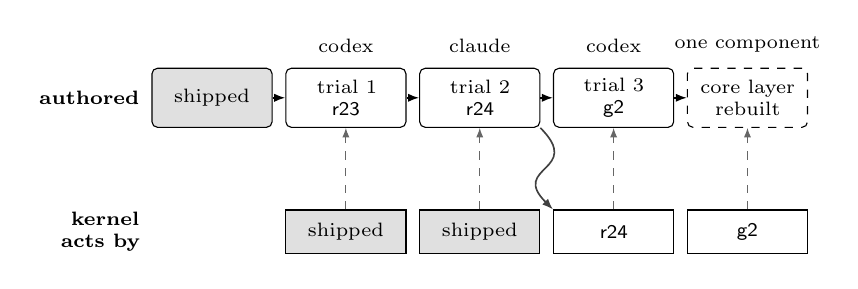
\begin{tikzpicture}[
  font=\scriptsize,
  x=1cm, y=1cm,
  impl/.style={draw, rounded corners=2pt, align=center, inner sep=2.5pt,
               text width=1.35cm, minimum height=7.5mm},
  ship/.style={impl, fill=black!12},
  regr/.style={impl, fill=white},
  exec/.style={draw, align=center, inner sep=2.5pt, text width=1.35cm,
               minimum height=5.5mm},
  flow/.style={-{Latex[length=1.4mm]}, semithick},
  op/.style={-{Latex[length=1.2mm]}, draw=black!60, dashed},
  hdr/.style={font=\scriptsize\bfseries, align=right},
]

% --------------------------------------------------- row 1: authored by
\node[hdr, anchor=east, text width=1.3cm] at (-0.35,0) {authored};
\node[ship] (g0) at (0.45,0) {shipped};
\node[regr] (t1) at (2.15,0) {trial 1\\\textsf{r23}};
\node[regr] (t2) at (3.85,0) {trial 2\\\textsf{r24}};
\node[regr] (t3) at (5.55,0) {trial 3\\\textsf{g2}};
\node[regr, dashed] (t4) at (7.25,0) {core layer\\rebuilt};

\draw[flow] (g0) -- (t1);
\draw[flow] (t1) -- (t2);
\draw[flow] (t2) -- (t3);
\draw[flow] (t3) -- (t4);

\node[font=\scriptsize, anchor=south] at (2.15,0.45) {codex};
\node[font=\scriptsize, anchor=south] at (3.85,0.45) {claude};
\node[font=\scriptsize, anchor=south] at (5.55,0.45) {codex};
\node[font=\scriptsize, anchor=south] at (7.25,0.45) {one component};

% ------------------------------------------------- row 2: executed by
\node[hdr, anchor=east, text width=1.3cm] at (-0.35,-1.70)
  {kernel acts by};
\node[exec, fill=black!12] (e1) at (2.15,-1.70) {shipped};
\node[exec, fill=black!12] (e2) at (3.85,-1.70) {shipped};
\node[exec] (e3) at (5.55,-1.70) {\textsf{r24}};
\node[exec] (e4) at (7.25,-1.70) {\textsf{g2}};

\draw[op] (e1) -- (t1);
\draw[op] (e2) -- (t2);
\draw[op] (e3) -- (t3);
\draw[op] (e4) -- (t4);

% the transfer of the operational role: trial 2 becomes the executor
\draw[flow, draw=black!75] (t2.south east)
  .. controls +(0.55,-0.55) and +(-0.55,0.55) .. (e3.north west);

\end{tikzpicture}

\caption{Recursive self-hosting lineage at frozen identity
\texttt{900b6594}. The lower row records which implementation executed
each generation's kernel operations.}
\label{fig:lineage}
\end{figure}

\begin{table}[t]
\centering\small
\caption{Reconstructions at the final frozen identity
\texttt{900b6594}, each sealed as a claim whose own gate re-earns the
verdict. No row has been reproduced by an external operator.}
\label{tab:trials}
\begin{tabular}{@{}llll@{}}
\toprule
trial & sealed claim & producer & executed by \\
\midrule
1 & \texttt{61d77f1f} & codex & shipped \\
2 & \texttt{29b185a8} & claude & shipped \\
3 & \texttt{2568e7d4} & codex & trial 2 \\
\bottomrule
\end{tabular}
\end{table}

The system was decomposed into 21 components and reconstructed in
dependency order, each component's producer receiving already-reconstructed
dependencies as context and never the original component. Assembled
implementations were then judged against the unchanged whole-system
identity with all 37 generated modules substituted.

At the final frozen identity \texttt{900b6594}, three reconstructions
qualified (Table~\ref{tab:trials}): one from each producer family, and a
third in which every component was authored blind by one family while
every kernel operation --- sealing, sandboxing, rebuilding, computing
identities --- was executed by the \emph{other} family's reconstructed
code, with no shipped code in the loop. That third result is the one
that answers \RQ{2}, because it transfers the operational role rather
than only the implementation: the tool performing the work is itself a
reconstruction. Its own recursive step then exercised the operational
interface directly: using the reconstruction's own command-line tool, a
component claim was exported blind, imported into a fresh workspace,
rebuilt through a producer, and found to carry the identity of the
original, with the parent verifying the child. We state the scope of
that step precisely, because it is easy to overstate. It rebuilds
\emph{one component} --- the core layer, identity \texttt{4c2abcbf} ---
and not a further whole-system generation. What it establishes is that a
reconstruction can perform the export, rebuild and verification
operations the method requires, not that a fourth complete system was
grown.

Each qualifying reconstruction is sealed as a claim whose own acceptance
procedure re-executes the conditions, so the verdict is re-earned rather
than asserted. A claim cannot seal unless its obligations pass, and two
non-qualifying trials in this series have no sealed manifest, which we
verified directly. The construction also refused a seal over a boundary
whose own obligations named a path outside the claim, which was then
fixed.

\paragraph{Implementation diversity.} The measured population is eight
complete implementations: \emph{seven independent reconstructions}
(three codex, four claude) together with the shipped implementation as a
reference point. Similarity figures between reconstructions are computed
over the seven; the shipped tree enters only where it is named.

Among the seven, mean pairwise text similarity is $0.123$ across producer
families, $0.317$ within the codex family and $0.201$ within the claude
family. Of the 37 modules present in every implementation, 32 take a
distinct syntactic shape in every reconstruction; the five that converge
are package initialization files and the top-level entry point, which
contain almost nothing to write. Reconstruction size is bimodal by
family: 4{,}384 to 4{,}842 lines for codex and 8{,}381 to 8{,}638 for
claude. The shipped implementation, scored against the seven, is the
least typical member of its own admitted class at similarity $0.074$. Measured with comments, docstrings and
layout normalized away, the same figures are $0.198$, $0.349$ and $0.290$;
we report both channels because the raw figure credits prose differences
as implementation diversity and the normalized figure does not.

The identity is therefore not accidentally stable. It survived three
complete replacements of the bytes it names, with the replacements
measurably dissimilar to one another and to the original.

These are textual measures, and textual dissimilarity is weaker evidence
than it may appear. It establishes that the reconstructions are not
copies, which is what bears on memorization. It does not establish that
they embody different algorithms, and we make no such claim: two
implementations may share an approach and still share little text.
Functional and structural diversity measures would settle this, and we
have not applied them.

\paragraph{The cost of the result.} The final count of three was reached
only after the count was reset to zero five times by adopted boundary
changes, and once by a ruling that a trial whose authoring predated a
comment-only identity change could not count under a strict reading of
the no-intervening-change condition. One reset surrendered an already
qualifying trial in order to adopt a requirement the authors judged more
valuable than the count. A reader who learns only the final figure has
been misled about the method's cost: the three qualifying reconstructions
are the end of a sequence of approximately two dozen, most of which
failed, and each failure that was adopted as a repair invalidated the
results before it.

\begin{table}[t]
\centering\small
\caption{Reconciliation of the reconstruction counts used in this
paper. The populations are nested subsets of one series, not independent
experiments.}
\label{tab:accounting}
\begin{tabular}{@{}rp{0.33\textwidth}@{}}
\toprule
$n$ & population \\
\midrule
26 & whole-system reconstructions with a recorded producer ledger,
     across all boundary versions. The basis for the timing and retry
     figures of \S\ref{sec:design}. \\
8  & complete reconstructions retained as artifacts and used for the
     diversity measurements, drawn from several boundaries. Includes the
     shipped implementation as a reference point. \\
7  & the same set excluding the shipped implementation: the
     reconstructions only, used for the per-component agreement
     gradient in the appendix. \\
3  & reconstructions qualifying at the final frozen identity
     \texttt{900b6594} under every condition of \S\ref{sec:tmt} except
     the external leg. The basis for Table~\ref{tab:trials}. \\
\bottomrule
\end{tabular}
\end{table}

\subsection{Specification repair during self-hosting}
\label{sec:repair}

\begin{table*}[t]
\centering\small
\caption{Representative adopted obligations, the failure that selected
each, and the evidence since adoption. Nineteen obligations are recorded
in total; the project's revision lineage contains 34 recorded
transitions.}
\label{tab:repairs}
\begin{tabular}{@{}p{0.26\textwidth}p{0.30\textwidth}p{0.34\textwidth}@{}}
\toprule
obligation adopted & failure that selected it & evidence since adoption \\
\midrule
Pattern expansion applies to pinned inputs, not only generated outputs
  & A reconstruction expanded globs in one field and read the other
    literally; refused at 21\,s
  & No recurrence across the following six reconstructions \\
The reconstruction workspace recipe is TOML
  & A reconstruction wrote canonical JSON into the recipe file,
    self-incompatible with its own format
  & No recurrence across the following six reconstructions \\
A component record round-trips between packaging and deep audit
  & A reconstruction sealed records as \texttt{\{component, root\}}
    while its own deep audit read an \texttt{input} key
  & Steering confirmed 4/4: the packaging layer passed first-attempt in
    the next four reconstructions \\
Components resolve by identity, never by physical nesting
  & Two independently written walkers in different families made the
    same assumption; 2 of 4 incidence cross-family
  & The transitivity fixture now stages components flat mid-battery \\
The sandbox must permit a real gate (user lookup)
  & A reconstruction passed identity but failed as \emph{auditor}: its
    deny-default sandbox refused a user lookup the repository gate needs
  & Steering confirmed 1/1: the next reconstruction passed both the run
    layer and the repository audit, becoming the first qualifier in its
    family \\
A pattern may select the empty set
  & A reconstruction raised on a glob matching no file, where the chain's
    uniform early-layer patterns legitimately select nothing
  & The next reconstruction took the empty selections without complaint \\
A declared data dependency re-earns its content match
  & A forged attribution passed every verification verb in every
    reconstruction, the shipped implementation included
  & Refusal now names the attribution; the shipped implementation
    required a fix \\
The chain build is incremental (doubling cost bounded)
  & A reconstruction walked ancestor links once per reaching path:
    measured doubling ratio ${\approx}95$ against 2.1--3.5 for
    conforming implementations, with a $2^{K}$ model fitting the
    interpolated point to 1\%
  & First obligation adopted on a time axis \\
\bottomrule
\end{tabular}
\end{table*}

Failures were classified before any repair was drafted.
Table~\ref{tab:repairs} gives representative entries from the 19 adopted
obligations. The recurring classes were: workspace and filesystem
assumptions (pattern expansion, empty selections, flat versus nested
staging); sandbox policy, where a reconstruction's own confinement
profile was simultaneously strict enough to pass its tests and too
strict to run the system's real acceptance gate; record and format
round-trips between components written at different layers; composed
verdicts that did not re-earn their parts; and resource growth.

Three features of this record bear on \RQ{4}.

First, the \emph{sequence of newly discovered failures per generation
declined} across the codex arc, counted by the project at the time as
3, 3, 3, 2, 1, 0 for successive reconstructions. We report these as the
authors' classification rather than as a mechanically derived series;
the underlying per-revision records exist, but the counts were not
emitted by a script.

Second, several obligations have direct post-adoption evidence that they
steered subsequent reconstructions, noted in Table~\ref{tab:repairs}.
The clearest is the sandbox obligation: the reconstruction immediately
following its adoption passed both the component gate and the
whole-repository audit, becoming the first qualifying reconstruction from
the claude family after seven consecutive refusals.

Third, and in the other direction, the second producer family's arc shows
what repair does \emph{not} buy. Seven consecutive reconstructions from
that family were each refused by exactly one defect, each defect deeper
in the system than the last, with three adopted obligations in between.
Repair moved the failure rather than eliminating it, until the eighth
reconstruction qualified. We cannot distinguish "the obligations were
progressively completed" from "the family's failures were enumerable and
we exhausted them" on this evidence.

\paragraph{Obligations not adopted.} Three candidate obligations were
drafted and rejected after measurement contradicted the diagnosis they
encoded: one attributed a failure to a deduplication key, which
measurement falsified; one assumed silent truncation where the
implementation in fact raised; one isolated a mechanism that could not be
encoded as a fixture and was accepted as already caught elsewhere. We
record these because the discipline they represent is load-bearing: an
authorization step authorizes an intent, and an intent resting on a wrong
diagnosis produces an obligation that refuses conforming
implementations.

\paragraph{Resource obligations.} Functional obligations accept
implementations with arbitrarily poor asymptotics, and absolute time
bounds cannot be committed to a portable identity because they describe
a machine rather than a program. Growth ratios can. For an operation
parameterized by scale $K$, measured twice on the same host in the same
run,
\begin{equation}
t(2K)/t(K) \;\le\; c,
\label{eq:ratio}
\end{equation}
the host's constant factor divides out and what remains constrains the
algorithm. A slow linear implementation on slow hardware passes; a fast
exponential one fails everywhere. This form caught the traversal defect
in Table~\ref{tab:repairs} and a corresponding space defect, in which a
copy procedure duplicated shared ancestors once per reaching path and a
dependency store grew exponentially in chain depth, reaching
approximately 23\,GB for a 20-layer chain in ordinary use. The declared
envelope bounds doubling on the recursion-bearing axes at $\times 8$
against a measured conforming band of 1.1--3.5. The limitation is that a
ratio constrains the exponent only at the scales measured.

\subsection{Consumer substitution}
\label{sec:substitution}

This experiment is the cleanest answer to \RQ{3} and the sharpest
illustration of the gap between test-based and behavioral equivalence.

A configuration parser $D$ was sealed with a deliberately partial
boundary $C_0$ that pins word-valued, distinct-key assignments and the
empty document, leaving numeric coercion and duplicate-key meaning
unspecified. A consumer $P$ was sealed separately; it parses a document
with a repeated \texttt{port} key and doubles the resulting value,
expecting 160. $P$'s recipe makes the parser a generated file, so $P$'s
identity commits to the contract and never to any parser's bytes, and a
candidate parser is judged by auditing $P$ with that candidate
substituted.

Six blind reconstructions of $D$ from $C_0$ alone were produced across
two families and six models. All six were admitted by $C_0$. All six had
distinct build digests. \textbf{None kept the consumer working.}

The failure was not six independent mistakes. Every reconstruction chose
last-wins for duplicate keys, which the consumer needed, and kept values
as strings, which broke it: the consumer's \texttt{cfg["port"] * 2}
evaluated to \texttt{"8080"} by string repetition. The boundary was
silent about coercion and both families' priors filled the silence the
same way, on the side the consumer could not use.

The consequence for the method is stronger than the consequence for the
parser. Six independent implementations that agree with one another all
broke the consumer identically, so no amount of cross-checking
reconstructions against each other would have surfaced the defect. Only
the consumer did. This is the correlated-failure
result~\cite{knight1986} in a setting where diversity is cheap, and it
bounds what differential comparison between reconstructions can
establish.

Adding the two obligations the consumer relied upon --- numeric values
coerce, duplicate keys are last-wins --- produced a tightened boundary
$C_1$. Re-running the same six producers against $C_1$: all six were
admitted and all six kept the consumer working. The difference is two
pinned lines. One reconstruction needed a second attempt.

\subsection{External software: \texttt{jq}}
\label{sec:jq}

\begin{figure*}[t]
\centering
% Figure 4 --- Behavioral divergence before and after repair, measured
% two ways on the SAME data. Editable TikZ source, hand-plotted (no
% external data toolchain) from:
%   research/external/jq/baseline/rate_comparison.json
%   research/external/jq/rate-metric-findings.md
% Left panel: the aggregate per-sample count, with the dispersion that
% made it uninformative. Right panel: the paired per-probe comparison.
% The figure exists to show that the measurement design, not the data,
% decided the conclusion.
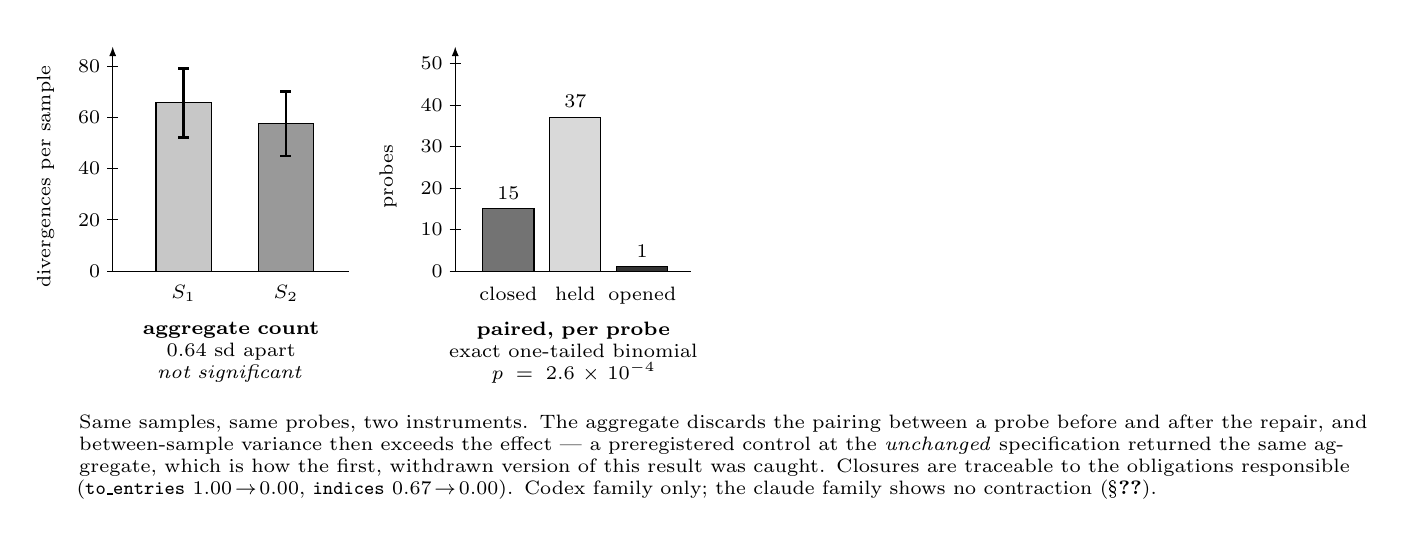
\begin{tikzpicture}[font=\scriptsize]

% ===================================================== LEFT: aggregate
\begin{scope}[xshift=0cm]
  \def\H{2.6}            % axis height
  \def\S{0.0325}         % units per divergence  (80 -> 2.6)
  \draw[-{Latex[length=1.2mm]}] (0,0) -- (0,\H+0.25)
    node[above, font=\scriptsize] {};
  \draw (0,0) -- (3.0,0);
  \foreach \v in {0,20,40,60,80}
    \draw (-0.07,\v*\S) -- (0.07,\v*\S) node[left, xshift=-3pt] {\v};
  \node[rotate=90, anchor=south, yshift=0.52cm, xshift=-0.1cm]
    at (-0.1,\H/2) {divergences per sample};

  % bars: S_1 = 65.7 +- 13.5 ; S_2 = 57.6 +- 12.6
  \fill[black!22] (0.55,0) rectangle (1.25,{65.7*\S});
  \draw          (0.55,0) rectangle (1.25,{65.7*\S});
  \fill[black!40] (1.85,0) rectangle (2.55,{57.6*\S});
  \draw          (1.85,0) rectangle (2.55,{57.6*\S});

  % error bars (sd)
  \draw[thick] (0.90,{(65.7-13.5)*\S}) -- (0.90,{(65.7+13.5)*\S});
  \draw[thick] (0.83,{(65.7-13.5)*\S}) -- (0.97,{(65.7-13.5)*\S});
  \draw[thick] (0.83,{(65.7+13.5)*\S}) -- (0.97,{(65.7+13.5)*\S});
  \draw[thick] (2.20,{(57.6-12.6)*\S}) -- (2.20,{(57.6+12.6)*\S});
  \draw[thick] (2.13,{(57.6-12.6)*\S}) -- (2.27,{(57.6-12.6)*\S});
  \draw[thick] (2.13,{(57.6+12.6)*\S}) -- (2.27,{(57.6+12.6)*\S});

  \node at (0.90,-0.28) {$S_1$};
  \node at (2.20,-0.28) {$S_2$};
  \node[anchor=north, text width=3.0cm, align=center] at (1.5,-0.52)
    {\textbf{aggregate count}\\$0.64$ sd apart\\\emph{not significant}};
\end{scope}

% ======================================================== RIGHT: paired
\begin{scope}[xshift=4.35cm]
  \def\H{2.6}
  \def\P{0.0527}         % units per probe (50 -> 2.6)
  \draw[-{Latex[length=1.2mm]}] (0,0) -- (0,\H+0.25);
  \draw (0,0) -- (3.0,0);
  \foreach \v in {0,10,20,30,40,50}
    \draw (-0.07,\v*\P) -- (0.07,\v*\P) node[left, xshift=-3pt] {\v};
  \node[rotate=90, anchor=south, yshift=0.52cm, xshift=-0.1cm]
    at (-0.1,\H/2) {probes};

  % closed 15, held 37, opened 1
  \fill[black!55] (0.35,0) rectangle (1.00,{15*\P});
  \draw           (0.35,0) rectangle (1.00,{15*\P});
  \node[anchor=south, font=\scriptsize] at (0.675,{15*\P}) {15};

  \fill[black!15] (1.20,0) rectangle (1.85,{37*\P});
  \draw           (1.20,0) rectangle (1.85,{37*\P});
  \node[anchor=south, font=\scriptsize] at (1.525,{37*\P}) {37};

  \fill[black!80] (2.05,0) rectangle (2.70,{1*\P});
  \draw           (2.05,0) rectangle (2.70,{1*\P});
  \node[anchor=south, font=\scriptsize] at (2.375,{1*\P}) {1};

  \node[anchor=north, align=center] at (0.675,-0.08) {closed};
  \node[anchor=north, align=center] at (1.525,-0.08) {held};
  \node[anchor=north, align=center] at (2.375,-0.08) {opened};
  \node[anchor=north, text width=3.2cm, align=center] at (1.5,-0.52)
    {\textbf{paired, per probe}\\exact one-tailed binomial\\$p=2.6\times10^{-4}$};
\end{scope}

% ---------------------------------------------------------------- note
\node[anchor=north west, text width=16.6cm, align=left,
      font=\scriptsize]
  at (-0.55,-1.70)
  {Same samples, same probes, two instruments. The aggregate discards
   the pairing between a probe before and after the repair, and
   between-sample variance then exceeds the effect --- a preregistered
   control at the \emph{unchanged} specification returned the same
   aggregate, which is how the first, withdrawn version of this result
   was caught. Closures are traceable to the obligations responsible
   (\texttt{to\_entries} $1.00\!\to\!0.00$,
   \texttt{indices} $0.67\!\to\!0.00$). Codex family only; the claude
   family shows no contraction (\S\ref{sec:jq}).};

\end{tikzpicture}

\caption{Behavioral divergence before and after repair, measured two ways
on the same samples and probes.}
\label{fig:divergence}
\end{figure*}

The external arm applies the method to software the authors did not
write, where independently developed implementations already exist and
can serve as a divergence surface. The target is \texttt{jq} 1.8.1, with
\texttt{gojq} 0.12.19 and \texttt{jaq} 3.1.1 as oracles. The oracles
adjudicate and are never used as acceptance criteria.

\paragraph{The premise, measured without model spend.} Running the
official \texttt{jq} corpus of 522 parseable cases against all three
implementations, all three return the same verdict on 373 and differ on
149, a disagreement rate of \textbf{28.5\%}. Of the 373 agreements, 332
are cases all three pass and 41 are cases all three fail identically.
Per-implementation pass counts on \texttt{jq}'s own corpus are 479, 408
and 337. An officially maintained
test corpus is therefore measurably insufficient to pin the behavior of
its own language, as judged by independent human
reimplementations. Approximately 43 cases fail even for the reference
implementation under a plain runner and are excluded as harness
artifacts. The initial specification $S_0$ is the 465-case evaluation-core
slice.

\paragraph{Generation 1: the degenerate member.} The first blind
reconstruction converged on the first attempt, passed 465 of 465, and
verified clean: a member of $\widehat{\mathcal{I}}(S_0)$. On 1{,}395
seeded probes drawn from outside the corpus it agreed with the reference
on 587 and raised an error on the remaining 808. The reason is in the
implementation's own header, which states that the supplied specification
is an extensional set of observations and that the artifact is not a
general interpreter. It is a 465-entry lookup table with careful input
normalization. Proposition~\ref{prop:ext} is not a hypothetical: given a
finite corpus and nothing else, a competent producer built the cheapest
member of the admitted class and documented that it had done so. On the
same probe set the human implementations split from the reference on 296
of 1{,}395, which is live divergence territory outside the corpus.

\paragraph{Repairs.} Two revisions followed, each signed. $S_1$ added 16
metamorphic and computed laws over inputs seeded from entropy at
evaluation time, validated on three fresh seeds against the reference.
$S_2$ added 28 error-condition laws requiring that generated ill-typed
inputs raise, each condition first verified unanimous across all three
implementations, validated on five fresh seeds. Three further candidate
laws were \emph{rejected} by that validation before adoption, because the
reference's refusals proved value-dependent rather than type-dependent:
it reverses the number $0$ to the empty list but raises on $5$, since its
definition routes through a length that is zero in the first case. Had
those three been committed as drafted they would have refused conforming
implementations.

\paragraph{Preregistered predictions.} Of the predictions recorded before
the first workspace opened, one was supported, one falsified, one
returned nothing.

\emph{Concentration (supported).} The generation surfaced 107 distinct
divergent probes, of which 60 lie on the human-divergence surface:
56.1\% against a base rate of $340/1395 = 24.4\%$, an enrichment of
$2.30\times$. In the sharpest form, of the 19 probes where
reconstructions from \emph{both} families diverge from the reference, 17
(89\%) are probes where a human reimplementation also disagrees.
Independent machine priors and independent human teams locate the same
silence.

\emph{Recall (falsified).} The prediction was that sampled
reconstruction would surface at least 30\% of the human-divergence
surface. Measured: \textbf{17.6\%} (60 of 340 probes). Three codex
samples reached 15.0\%, and adding an entire second producer family moved
this to 17.6\%. The refined finding is more useful than the original
guess: the silence that two frontier priors can jointly see is
substantially narrower than the silence that demonstrably exists.
Sampled reconstruction finds a concentrated and high-value fraction of
the divergence surface, not all of it.

\emph{Novel ambiguity (none found).} Under a strict criterion --- a
both-succeed value divergence, off the human-divergence surface, flagged
by at least two independent samples --- the measured count is
\textbf{zero}. The off-surface multi-sample set consists entirely of
cases where reconstructions succeed and the reference and both human
implementations raise, which is a defect class rather than novel
ambiguity. With contamination as heavy as this target's, the priors
reproduce documented semantics well and fail where the reference is
silent about errors.

\paragraph{Did the repair reduce divergence?} This question produced the
arm's most transferable methodological result, and we report the error
along with the correction.

An initial reading compared aggregate divergence counts per sample and
appeared to show a 25\% reduction. A preregistered control at the
\emph{unchanged} specification returned the same aggregate: pooled by
boundary, $65.7 \pm 13.5$ before against $57.6 \pm 12.6$ after, a
difference of 0.64 standard deviations. Between-sample variance exceeded
the effect, and the claim was withdrawn within the hour.

Re-measured as a paired per-probe comparison --- the same probe before
and after, where a probe counts as consistently divergent if it diverges
in at least two thirds of samples --- the effect is present. At
$n=7$ and $n=5$ samples: \textbf{15 probes closed, 37 held, 1 opened},
exact one-tailed binomial $p = 2.6 \times 10^{-4}$. The effect
strengthened as samples were added, from 10:1 and $p = 5.9 \times 10^{-3}$
at the smaller sample. Closures are traceable to the obligations
responsible, with \texttt{to\_entries} moving from a divergence rate of
1.00 to 0.00 and \texttt{indices} from 0.67 to 0.00, both named
explicitly in the error laws. Figure~\ref{fig:divergence} shows both
measurements on the same data.

The aggregate discards the pairing between a probe before and after the
repair, and the pairing is where the signal is. Same samples, same
probes, two instruments, opposite conclusions.

\paragraph{A negative cross-family result.} The contraction above is
measured on the codex family. On the claude family it does not replicate:
paired at $n=1$ per boundary, 12 probes closed, 22 held and 12 opened, a
sign test of $p = 0.58$ and no contraction at all.

The class decomposition explains this, and the explanation is measurable.
Divergence falls into classes, and the families have different profiles:
excess permissiveness accounts for 54\% of the codex family's divergence
and 18\% of the claude family's. The $S_2$ repair was 28 error laws,
aimed squarely at permissiveness, and permissiveness fell in both
families. But a repair that addresses a class constituting half of one
family's divergence and a fifth of another's will move one aggregate and
not the other. The repair did what it was designed to do; the measurement
of whether a specification improved is not answerable from one family's
aggregate.

We report this as a negative result and not as a resolved one. The claude
leg is $n = 1$ and carries no statistical weight on its own. The account
is falsifiable and the test is specified in advance: a pending revision
targets the value-divergence class, and the account predicts that a fresh
claude sample's value-divergence count will fall while its permissiveness
count stays flat.

\paragraph{Byproducts.} The probe batteries incidentally surfaced three
undocumented divergences in the ecosystem, each reproducible with a
single command: the reference returns an empty list where both
reimplementations raise; one reimplementation fails to terminate on a
generated range over a string; and the reference itself fails to
terminate on a large string repetition, apparently building the result
eagerly. Two of the three are in the reference implementation. These are
byproducts of the method rather than contributions of this paper.

\paragraph{An open decision.} Of the programs that diverge consistently
at both boundaries, 19 reduce to four classes. Six differ only in error
message text, which the project's precedent leaves unpinned. Nine have a
single reimplementation as the outlier and admit a mechanical consensus
resolution. Three constitute a genuine election: indexing an object by a
string key where the reference returns null and \emph{both}
reimplementations raise. Pinning the reference's behavior requires
members to replicate a permissive edge that two independent
implementations treat as an error; pinning the majority produces a
specification that refuses the artifact it was recovered from. This
decision is unresolved at the time of writing.

\subsection{Consolidated findings}
\label{sec:consolidated}

\begin{table*}[t]
\centering\small
\caption{Findings by level of support. No row has been independently
reproduced by an operator outside the authors' environment.}
\label{tab:findings}
\begin{tabular}{@{}p{0.055\textwidth}p{0.42\textwidth}p{0.44\textwidth}@{}}
\toprule
& finding & support \\
\midrule
\multicolumn{3}{@{}l}{\textbf{Demonstrated}}\\
\RQ{1}
 & Independent reconstructions satisfy a frozen specification and are
   measurably dissimilar: cross-family similarity 0.123, 32 of 37
   modules distinct in every reconstruction.
 & Eight complete reconstructions measured; three qualifying at one
   identity; instrument reproduces a prior reading to $\pm0.003$. \\
\RQ{3}
 & Test-based admission does not imply substitutability: 6/6
   reconstructions admitted, 0/6 usable by the consumer, failing
   identically.
 & Six reconstructions, two families, six models; repair verified by
   re-running the same producers (6/6 usable). \\
\RQ{3}
 & A finite test corpus admits memorization, and a producer realizes it:
   465/465 conformance by a 465-entry lookup table.
 & Implementation source preserved; 587 agreements and 808 refusals on
   1{,}395 novel probes. \\
\RQ{5}
 & An officially maintained corpus is insufficient to pin its own
   language: 28.5\% three-way disagreement.
 & Full corpus against three implementations; no model spend. \\
\midrule
\multicolumn{3}{@{}l}{\textbf{Laboratory-only}}\\
\RQ{2}
 & A reconstruction can perform the operations that produce the next
   generation, preserving identity.
 & One lineage; kernel acts executed by a prior reconstruction; a
   further generation landed the same identity. Authors' hardware. \\
\RQ{4}
 & Witnessed failures converted into obligations reduce consequential
   divergence: 15 closed against 1 opened,
   $p = 2.6\times10^{-4}$.
 & Paired per-probe, codex family, $n=7$/$n=5$. Correlated probes;
   analysis specified after an initial instrument failure. \\
\RQ{4}
 & Newly discovered failures per generation declined (3,3,3,2,1,0).
 & Authors' classification, not mechanically derived. \\
\midrule
\multicolumn{3}{@{}l}{\textbf{Negative}}\\
\RQ{4}
 & The divergence reduction does not replicate in the second producer
   family: 12 closed, 12 opened, $p=0.58$.
 & $n=1$ per boundary. Class decomposition offers a falsifiable
   explanation. \\
\RQ{5}
 & Sampled reconstruction recovers only 17.6\% of the known human
   divergence surface, against a predicted $\ge 30\%$.
 & Preregistered and falsified; a second producer family added 2.6
   points. \\
\RQ{5}
 & No novel behavioral ambiguity was found (strict criterion: zero).
 & Below the instrument's sensitivity on a heavily contaminated target. \\
 & An aggregate divergence count is unable to detect the repair effect
   it was first used to claim.
 & Preregistered control at an unchanged specification refuted the
   original claim; it was withdrawn. \\
\midrule
\multicolumn{3}{@{}l}{\textbf{Open}}\\
 & External reproduction by an independent operator.
 & Protocol and signed-receipt format specified; nothing returned. \\
 & Whether repair completes a specification or merely relocates its
   failures.
 & Seven successive single-defect refusals in one family are consistent
   with both readings. \\
 & Cost relative to any alternative method.
 & No comparative cost study exists. \\
\bottomrule
\end{tabular}
\end{table*}

Table~\ref{tab:findings} separates what the evidence demonstrates, what
holds only within our environment, what came out negative, and what
remains open.

\section{Discussion}
\label{sec:discussion}

\subsection{Specification as a persistent asset}

If a specification is sufficient to obtain a conforming implementation,
then the specification and not the implementation is the durable object.
This reframes a familiar problem. Software knowledge is ordinarily lost
when an implementation becomes unmaintainable, because the requirements
were never separable from the code that satisfied them. An executable
specification with a stable identity is separable by construction, and
our self-hosting result is evidence that the separation can hold through
complete replacement of the implementation.

The claim must be bounded carefully. Specification identity is not
semantic identity. An identity over $S$ names a declared experiment: two
specifications that ask the same behavioral question by different means
receive different identities, and identity equality asserts that the same
question is being asked, not that the answer is correct.
Section~\ref{sec:substitution} is the cautionary case, in which the
preserved specification was faithfully satisfied and nonetheless
insufficient for its only consumer.

\subsection{Applications}

Several applications follow, each requiring technical work this paper
does not supply.

\emph{Legacy reconstruction.} Where a system must be replaced and its
behavior is known only through the system itself, the method offers a
procedure: recover a specification from observed behavior, then
reconstruct against it and use divergence to find what the recovery
missed. The \texttt{jq} arm is a small instance. The required advance is
specification recovery from execution traces at scale, for which dynamic
invariant inference~\cite{ernst2007} is the natural input.

\emph{Compatibility and regression discovery.} Independent
reconstruction is a source of inputs on which conforming implementations
disagree, and such inputs are exactly the regression tests a suite is
missing. The required advance is automatic triage: our divergence
classes were assigned by hand.

\emph{Vendor independence.} A consumer holding a specification with a
credible reconstruction path has an exit option from any particular
implementation. The required advance is a consumer-side acceptance
boundary strong enough that substitution is safe, which
\S\ref{sec:substitution} shows is a distinct and stronger property than
component-level conformance.

\emph{Assurance for generated code.} The method converts "the model
wrote something that passes" into "the requirements are recorded,
re-earnable, and known to admit at least these implementations." The
required advance is cheaper obligations, since the ones here were written
by hand.

\subsection{Economic implications}

We state these as hypotheses, because no cost study supports them. Our
repository records a per-reconstruction envelope and some per-run
figures, and compares nothing against an alternative method.

If generating an implementation becomes inexpensive while maintaining a
reliable specification does not, then economic value should shift toward
whoever holds the specification and the authority to judge conformance
against it. Four effects would be measurable: migration cost when
replacing an implementation; dependence on a particular vendor; time to
discover an undocumented requirement; and reuse of acceptance criteria
across implementation generations. Plausible business models follow ---
specification auditing, reconstruction infrastructure, continuous
behavioral verification --- but a model is not a measurement, and the
determining quantity is the human adjudication cost per replacement,
which we have not measured.

We note one consideration that cuts against naive optimism. The scarce
asset in this scheme is a maintained acceptance contract, and whoever
governs it holds the power the implementations lose. Consolidating
specifications moves authority to the specification steward, which is a
different risk from vendor lock-in rather than an absence of one.

\subsection{Iterated reconstruction against strengthening specifications}

The loop of \S\ref{sec:discovery} can in principle be iterated:
reconstruct, find divergence, strengthen, reconstruct again. Our results
are consistent with this accumulating knowledge while implementation
strategies vary freely, and the self-hosting arc is the longest instance
we have, at roughly two dozen reconstructions and nineteen adopted
obligations.

It should not be read as autonomous self-improvement. Every adopted
obligation in this work required a human authorization step, the
diagnosis behind three candidate obligations was wrong and was caught
only by measurement, and a producer improving its own acceptance
boundary has no external check. The arrangement that produced our
results keeps authorization outside the loop deliberately.

\subsection{Substitutability, markets and intellectual property}

If implementations become substitutable under a specification, two
distinctions become practically important. The first is between
\emph{technical reconstructability} and the \emph{legal right} to
reproduce or distribute: that a conforming implementation can be
obtained from a specification says nothing about whether doing so is
permitted, and the specification may itself be derived from a protected
artifact. The second is between behavior and expression. Our method
operates on behavior, and the legal treatment of behavioral
reimplementation is jurisdiction-specific and outside our competence. We
flag these because the method's attractiveness as a means of escaping
lock-in makes them immediate, not because this paper resolves them.

\section{Limitations and Threats to Validity}
\label{sec:threats}

\paragraph{Acceptance criteria are finite and incomplete.} Every
obligation in this work is an executing program over finitely many
inputs, and Proposition~\ref{prop:ext} applies to any part of it that
compares fixed observations. A specification that admits an
implementation has established conformance to itself and nothing more.
Failure to detect a defect is not evidence that none exists; the
\texttt{jq} arm's zero novel-ambiguity result is a statement about our
instrument's sensitivity.

\paragraph{Blindness is declared, not enforced.} The harness does not
route the original implementation into the reconstruction workspace, and
the specification states explicitly that content cannot prove blindness.
Our indirect evidence is artifact dissimilarity, two unrelated producer
families, and a held-out battery outside the committed identity. A
producer that had memorized the target would be detected by none of
these with certainty.

\paragraph{Specification and probe population co-evolved.} The
obligations were authored by the method's designer and revised
repeatedly in response to the behavior of the two producer families used
to probe them. This is the correct way to develop a boundary and a
confound when measuring one. A specification authored independently of
the producers that probe it would be a stronger test, and we have not run
one.

\paragraph{The self-hosting arm was not preregistered.} It was conducted
as development. Its results are therefore measurements of a system under
repeated repair rather than the outcome of a design fixed in advance, and
the declining failure-per-generation series in particular is the authors'
classification of their own development history.

\paragraph{External target selection.} \texttt{jq} was chosen for having
multiple independent implementations and an official corpus, which makes
it informative about divergence and uninformative about agreement,
because it is heavily represented in producer training
data~\cite{sainz2023,carlini2023}. One target does not support claims
about external software generally.

\paragraph{Small samples and correlated observations.} The paired
divergence analysis rests on 7 and 5 samples in one family and 1 in the
other. Probes within a sample are not independent: they are drawn from
the same seeded battery and a single implementation defect affects many
at once. We report exact tests on the paired per-probe unit and treat the
result as exploratory. The analysis was specified after an initial
instrument failure, which is adaptive analysis and a real threat; the
control that refuted the first attempt was itself preregistered, which
partially mitigates it.

\paragraph{The probe population that measured the repair also selected
it.} The error-condition obligations of \S\ref{sec:jq} were drafted from
failures witnessed on the 1{,}395-probe battery, and the paired
before-and-after comparison was then computed on that same battery. The
measured contraction therefore demonstrates effective repair on the
population that motivated it, and does not establish generalization to
unseen behavior. A stronger design freezes the specification, discovers
failures on one probe collection, constructs repairs, and evaluates
fresh reconstructions against a collection never used for selection. We
did not run that design, and the result should be read accordingly.

\paragraph{Overfitting during repair.} Obligations drawn from observed
failures may encode the particular producers' habits rather than the
target's semantics. Three candidate obligations were rejected on exactly
this ground after measurement contradicted them, which indicates the
failure mode is live rather than hypothetical.

\paragraph{Continuous integration is not external reproduction.} Our
criteria are re-executed on platform configurations we do not
administer, which tests portability. It runs our workflow, on our
specification, triggered by us. It is not an independent operator
reproducing a result.

\paragraph{No external reproduction exists.} This is the limitation a
reader should weigh most heavily. The protocol's own M2 leg, applied to
the self-hosting results, is incomplete in the technical sense of
\S\ref{sec:tmt}: a hard condition is declared and unmeasured. A protocol
and signed-receipt format for an external operator are specified in
advance, and nothing has been returned. Two records in the repository
named for the outside re-earn are same-host dry runs of that instrument,
not external replications. Every self-hosting result here is a
laboratory result.

\paragraph{No baseline comparison.} We did not run differential testing,
property-based testing, or synthesis tooling as alternative means of
finding the defects reported here, so we make no claim that
reconstruction finds them more cheaply or more completely than existing
techniques would.

\paragraph{Three generations is not an induction.} Nothing in the
machinery references generation depth. A lineage that held three times
may fail the fourth.

\section{Conclusion}
\label{sec:conclusion}

Reproducibility, as the field has developed it, preserves computational
artifacts: given the same inputs, recover the same bytes. We asked a
different question --- whether the requirements a system satisfies are
sufficient to obtain a new implementation that satisfies them too --- and
found it to be both answerable and productive.

The Three-Machine Test separates two claims that are ordinarily
conflated: that an artifact and its verdicts survive transport, and that
the disclosed requirements determine the artifact. The second is the one
that matters for generated software, and it is testable. A 21-component
system was reconstructed from its own committed requirements by two
unrelated producer families, with measured cross-family similarity of
0.123 and 32 of 37 modules structurally distinct in every
reconstruction. In one case a reconstruction then performed the kernel
operations for the following generation under the same identity, and its
own recursive step rebuilt and verified one component claim --- a
demonstration that the operational interface survives reconstruction,
not that a fourth complete system was grown.

Used repeatedly, reconstruction is also an instrument for finding what a
specification failed to say. It located a finite corpus that admitted its
own memorization, a parser boundary that six independent implementations
satisfied and none could be substituted under, and a set of
error conditions in an external language that its official test suite
never stated. Converting those findings into obligations measurably
reduced consequential divergence in one producer family and measurably
did not in the other, for a reason the class decomposition explains and
a pending experiment can falsify.

The honest summary of the method's cost is that three qualifying
reconstructions were the end of a sequence of roughly two dozen, that the
count was reset five times by the repairs the failures earned, and that
no result here has been reproduced by anyone outside our environment. The
open question is therefore not whether independent reconstruction can
discover underspecification --- it did, repeatedly, including defects in
our own implementation and in the reference implementation of an
established tool --- but whether the adjudication it requires can be made
cheap enough to run continuously. That is a question about cost, and it
needs the measurement study this paper does not contain.

\balance
\section*{Artifact Availability}

The platform, all acceptance criteria, failure witnesses, generated
implementations retained as evidence, analysis scripts, preregistration,
signed revision records and ledgers are in the public
repository~\cite{reticuli}, at the immutable snapshot
\texttt{4c5ca38}; every figure and number here resolves at that commit.
The repository also carries an evidence map that ties each quantitative
claim in this paper to the artifact supporting it, and records for each
whether the number was re-derived from stored data, read from a dated
record, or reported by the authors without separately recoverable data. Reconstructed implementations are destroyed
after measurement by design, and the retained corpus is the set used for
the diversity measurements of \S\ref{sec:selfhost}.

Two disclosures. First, one early probe record was overwritten by a later
run that reused its path; because the probes are seed-determined and the
implementation source was preserved, the record was regenerated exactly,
matching the figures recorded at the time (587 agreements and 808
refusals over 1{,}395 probes). No other number in this paper depends on
a file that was overwritten. Second, no new producer runs, reconstructions
or external replays were performed for this manuscript; every result is
drawn from the recorded history of the project and was re-derived from
stored artifacts where a script existed to do so.

\bibliographystyle{plain}
\bibliography{references}

\appendix
\onecolumn

\section{The reconstruction procedure}
\label{app:procedure}

\paragraph{Decomposition.} The self-hosting target is decomposed into 21
components ordered by dependency. Each component declares the pinned
inputs its obligations read, the outputs a producer must supply, and the
components it depends on. The decomposition is part of the committed
material and therefore part of the identity.

\paragraph{Per-component reconstruction.} For each component in
dependency order, the harness materializes a workspace containing the
committed content only: the acceptance programs, fixtures, pinned
inputs, and the recipe. Already-reconstructed dependencies are placed in
the workspace as context, because an implementation of a higher layer
must import the lower layers it builds on. The original implementation
of the component under reconstruction is not present in the workspace at
any point.

A producer is then invoked on the workspace and its output sealed. If the
component's obligations fail, the producer is re-invoked with the failure
output, up to a per-component attempt limit. Attempt counts are recorded
and reported raw (\S\ref{app:measurements}); a reconstruction that needed
retries is not thereby disqualified, since the obligations are the
acceptance condition and not the number of attempts.

\paragraph{Whole-system judgment.} After all components are
reconstructed, the assembled tree is judged against the unchanged
whole-system identity with all 37 generated modules substituted for the
originals. This is a stronger condition than per-component acceptance:
each component passed its own obligations in isolation, and the assembled
system must additionally satisfy the system-level obligations, including
the recursive audit of the dependency chain.

\paragraph{The blindness protocol, and its limits.} Blindness means
exactly this: the harness does not place the original implementation in
the producer's workspace, and the producer is invoked with no reference
to it. It does not mean, and the protocol cannot establish, that the
producer has no prior exposure to the target. The supporting evidence is
indirect and reported in \S\ref{sec:selfhost}: measured artifact
dissimilarity, two unrelated producer families, and a held-out battery
maintained outside the committed identity. The specification states the
limitation directly: producer independence is recorded, never enforced,
because content cannot prove blindness.

\paragraph{The recursive step.} A qualifying reconstruction must also
perform the operations the system exists to perform. The step exports a
claim through the reconstruction's own command-line interface, imports it
into a fresh workspace, rebuilds its generated outputs through a
producer, and checks that the resulting identity equals the original and
that the parent verifies the child. In the generational trials, every
such operation is executed by a prior reconstruction rather than by the
shipped implementation.

The step operates on one component claim, by default the core layer, and
not on the whole system. It establishes that a reconstruction can drive
the export, rebuild and verification path. It does not establish that a
further complete system was grown.

\section{Verdicts sealed as claims}
\label{app:trialclaims}

A verdict recorded in a log is unverifiable. Each qualifying
reconstruction is therefore sealed as a claim whose own acceptance
procedure re-executes the conditions that qualified it: identity under
full substitution, the held-out battery, and the operational steps. A
claim cannot seal unless its obligations pass, so a non-qualifying trial
produces no sealed manifest. We verified this property directly during
the evidence audit for this manuscript: of seven trial directories, the
five qualifying ones carry a sealed manifest and the two non-qualifying
ones carry none.

The construction made one catch of its own before any trial sealed: it
refused a seal over a boundary whose acceptance obligations named a path
outside the claim, which was then corrected.

The regress this invites terminates deliberately. Judges are auditable by
the machinery they judge with, and the one operation that is never
automated is authorization. Adopting an obligation, and so moving an
identity, requires a human signature; every obligation discussed in this
paper carries one, recorded alongside the failure that selected it.

\section{Detailed measurements}
\label{app:measurements}

\subsection{Producer cost and timing}

Across 26 recorded whole-system reconstructions, each of 21 components:

\begin{center}\small
\begin{tabular}{@{}lrrr@{}}
\toprule
family & median wall-clock & range & per-component retries \\
\midrule
codex (\texttt{gpt-6-sol}) & 40 min & 27--211 min & 0--1 \\
claude (\texttt{sonnet})   & 186 min & 147--438 min & 0--4 \\
\bottomrule
\end{tabular}
\end{center}

The declared cost envelope for a whole-system claim is \texttt{usd =
40.0}, pinned from the project's own ledger history with headroom. The
codex family ran on a flat-rate plan and recorded zero metered spend
against that ceiling; the claude family likewise ran on a subscription
rather than metered API billing. Consequently the dollar figures in the
repository understate the market cost of these reconstructions, and we
make no cost claim from them (\S\ref{sec:discussion}).

\subsection{Implementation agreement per component}

Mean pairwise raw text similarity across the seven independent
reconstructions (the shipped implementation excluded), by component,
highest to lowest. The pattern of interest is that
agreement tracks obligation density, and that every failure witness
recorded during the trials occurred at a low-agreement component.

\begin{center}\small
\begin{tabular}{@{}lll@{}}
\toprule
component & agreement & note \\
\midrule
\texttt{\_kernel/core.py}      & 0.377 & most heavily pinned component \\
\texttt{feedback.py}           & 0.244 & \\
\texttt{\_kernel/seal.py}      & 0.238 & \\
\texttt{\_kernel/attest.py}    & 0.216 & \\
\texttt{\_kernel/recipe.py}    & 0.209 & \\
\texttt{\_kernel/identity.py}  & 0.197 & \\
\texttt{\_util.py}             & 0.182 & \\
\texttt{hooks.py}              & 0.144 & \\
\texttt{transfer.py}           & 0.140 & \\
\texttt{reference.py}          & 0.134 & \\
\texttt{\_cli/output.py}       & 0.131 & \\
\texttt{pack.py}               & 0.117 & witness: record round-trip \\
\texttt{\_kernel/run.py}       & 0.116 & witness: sandbox floor \\
\texttt{attest.py}             & 0.114 & \\
\texttt{\_cli/handlers.py}     & 0.111 & \\
\texttt{assess.py}             & 0.110 & \\
\texttt{render.py}             & 0.104 & \\
\texttt{record.py}             & 0.102 & \\
\texttt{authoring.py}          & 0.099 & \\
\texttt{\_kernel/crosscheck.py}& 0.090 & \\
\texttt{\_cli/parser.py}       & 0.088 & \\
\texttt{\_cli/views.py}        & 0.084 & \\
\texttt{reuse.py}              & 0.075 & \\
\texttt{launcher.py}           & 0.067 & \\
\texttt{\_cli/statusview.py}   & 0.066 & \\
\texttt{\_kernel/build.py}     & 0.064 & \\
\texttt{kernel.py}             & 0.061 & \\
\texttt{registry.py}           & 0.060 & witness: staging, resolution \\
\texttt{\_cli/report.py}       & 0.057 & \\
\texttt{heldout.py}            & 0.049 & \\
\texttt{\_cli/verbs.py}        & 0.046 & \\
\texttt{\_cli/dispatch.py}     & 0.024 & least constrained component \\
\bottomrule
\end{tabular}
\end{center}

Package initialization files and the top-level entry point are omitted;
they agree at 0.58--0.76 and contain almost nothing to write. We state
the relationship between agreement and obligation density as an
observation rather than a tested correlation: the components are not
independent observations, and obligation density was not assigned
experimentally.

\subsection{Diversity instrument}

The similarity figures in \S\ref{sec:selfhost} were produced by an
instrument fixed before the measurements reported here were taken, and
validated by reproducing an earlier reading of the project's own corpus.
On the raw channel it recovers that reading to within $0.003$ on seven of
eight per-reconstruction scores, with the eighth high by $0.0070$, and
reproduces the count of 32 of 37 components structurally distinct in
every reconstruction. It reports two channels: raw text, and text with
comments, docstrings and layout normalized away via syntax-tree
unparsing. The normalized channel runs 0.05 to 0.09 higher, because a
substantial part of what separates two reconstructions as text is prose.

\section{External arm detail}
\label{app:jq}

\subsection{Materials}

The corpus is the official \texttt{jq} 1.8.1 test suite, 522 parseable
cases, frozen with checksums. All three implementations return the same
verdict on 373 of them --- 332 passed by all three, 41 failed
identically by all three --- and differ on the remaining 149. The oracles are \texttt{jq} 1.8.1,
\texttt{gojq} 0.12.19 and \texttt{jaq} 3.1.1, also frozen. The oracles
adjudicate disagreement and are never used as acceptance criteria, so
that no obligation is defined by running a reference implementation
inside the gate.

The initial specification $S_0$ is the evaluation-core slice: the 465
cases exercising expression semantics, excluding regular expressions,
dates, input/output, modules and command-line flags, and excluding
approximately 43 cases that fail even for the reference implementation
under a plain runner. The carve rule is "the case drives only the
evaluator", applied by a tagger script and reviewed once.

\subsection{Obligation inventories}

$S_1$ adds 16 computed and metamorphic laws evaluated over inputs seeded
from entropy at evaluation time: indexing and length relations computed
independently by the checker; composition against sequencing; idempotence
of sorting; round-tripping of serialization; and concatenation length
additivity. Each was validated on three fresh seeds against the
reference before adoption.

$S_2$ adds 28 error-condition laws requiring that generated ill-typed
inputs raise, covering wrong-typed arguments to entry conversion,
transposition, joining and character conversion; malformed path arrays
given to path deletion and assignment; non-path expressions given to path
extraction; mismatched operand types for containment and indexing; and
arithmetic on incompatible types. Each condition was first verified
unanimous across all three implementations, and the battery validated on
five fresh seeds. A sanity guard accompanies the battery so that an
implementation refusing all inputs cannot satisfy it.

Three drafted laws were rejected before adoption because measurement
contradicted them. The reference's refusals for list reversal,
transposition and vacuous quantification proved value-dependent rather
than type-dependent; reversing the number $0$ yields the empty list while
reversing $5$ raises, because the definition routes through a length that
is zero in the first case. One candidate was abandoned entirely, its
refusal condition not being expressible as a property of types.

\subsection{Probe battery and per-sample results}

The differential battery is 1{,}395 deterministic seeded probes over
program and input pairs that the corpus does not contain, executed
against four implementations. The human-divergence surface is the 340
distinct probes on which \texttt{gojq} or \texttt{jaq} disagrees with
the reference, giving a base rate of $340/1395 = 24.4\%$; it was frozen independently of
any reconstruction.

\begin{center}\small
\begin{tabular}{@{}llrr@{}}
\toprule
boundary & sample & divergent probes & on human surface \\
\midrule
$S_1$ & codex 1 & 79 & 47 (59\%) \\
$S_1$ & codex 2 & 52 & 43 (83\%) \\
$S_1$ & codex 3 & 66 & 44 (67\%) \\
$S_1$ & pooled (distinct) & 92 & 51 (55\%) \\
$S_1$ & claude 1 & 34 & 26 (76\%) \\
\bottomrule
\end{tabular}
\end{center}

Of the 92 pooled codex divergences, 43 were flagged by all three samples,
19 by two and 30 by one, which indicates the battery measures structure
rather than noise. Of the 43 flagged by all three, 40 (93\%) lie on the
human-divergence surface.

The claude sample is 3{,}263 lines against the codex samples' 869, a
ratio of 3.8, which independently reproduces the family size signature
measured on the self-hosting corpus. It is also qualitatively different:
17 of its 34 divergences are cases where both implementations succeed
with different values, where the codex samples' divergences were
dominated by excess permissiveness.

\subsection{Divergence classes by family}

The class decomposition that explains the negative cross-family result in
\S\ref{sec:jq}:

\begin{center}\small
\begin{tabular}{@{}llrrr@{}}
\toprule
family & boundary & permissive & value split & sample error \\
\midrule
codex  & $S_1$ & 35.3 & 19.3 & 10.0 \\
codex  & $S_2$ & 27.5 & 13.0 &  8.0 \\
claude & $S_1$ &  6   & 17   & 11   \\
claude & $S_2$ &  5   & 20   &  9   \\
\bottomrule
\end{tabular}
\end{center}

Excess permissiveness is 54\% of the codex family's divergence and 18\%
of the claude family's. The $S_2$ repair targeted permissiveness, and
permissiveness fell in both families. The aggregate moved only for the
family in which that class dominates.

\subsection{The unresolved election}

Of the programs diverging consistently at both boundaries, 19 reduce to
four classes: six differing only in error message text, which project
precedent leaves unpinned; nine with a single reimplementation as the
outlier, admitting a mechanical consensus resolution; three constituting
a genuine election, where indexing an object by a string key returns null
in the reference and raises in both reimplementations; and one liveness
divergence recorded as a finding rather than pinned. The three-case
election is unresolved. Electing the reference requires members to
replicate a permissive edge two independent implementations treat as an
error; electing the majority produces a specification that refuses the
artifact it was recovered from.

\section{Reproduction}
\label{app:repro}

The repository contains the protocol for an independent operator to
re-earn a sealed trial, together with the signed-receipt format and a
continuous-integration workflow that checks a returned receipt against
the bundle's own public key. Re-earning a sealed trial claim requires the
checkout, the retained reconstruction lineage, and one audit command; it
executes the acceptance obligations and does not require a producer or
any model spend.

Reproducing a reconstruction from scratch requires a producer. The
expected cost is given in \S\ref{app:measurements}; because both families
were run on flat-rate plans, an operator billed per token should expect a
materially higher figure, and the declared envelope of \texttt{usd =
40.0} per whole-system claim is the project's own stated ceiling rather
than a measured market price.

No external operator has returned a receipt. The two records in the
repository named for this condition are same-host dry runs of the
instrument, retained to show the measurement path works, and each still
carries a placeholder note in place of an operator's signature.

\twocolumn


\end{document}
